% !TeX root = ../main.tex
% Add the above to each chapter to make compiling the PDF easier in some editors.

\chapter{Experiments}

In total, 5 experiments were conducted for this thesis. Two were quick proof-of-concept experiments to validate the initial speculation, two - pilot studies to determine values for some properties of the final experiment and test the process of sampling participants on \gls{wa} index, and one formal study to test \nameref{final_study}. 
The audio specialization tool used in all the pilots and final studies was Resonance Audio SDK for Unity with occlusion effect turned off.
Participants in all of the studies were asked for their consent, in case they were recorded.


\begin{comment}
\section{Prototypes/Proof of concept}

Initial motivation for this work was a question of whether sudden manipulations of buildings in \gls{vr} would cause uncomfortable experience for users (Fig. \ref{fig:a1unawareofa2actions}). Two prototypes were developed to test this speculation, these are described in the Buildings Popping Up and Moving Buildings paragraphs.

\begin{figure}
	\centering
	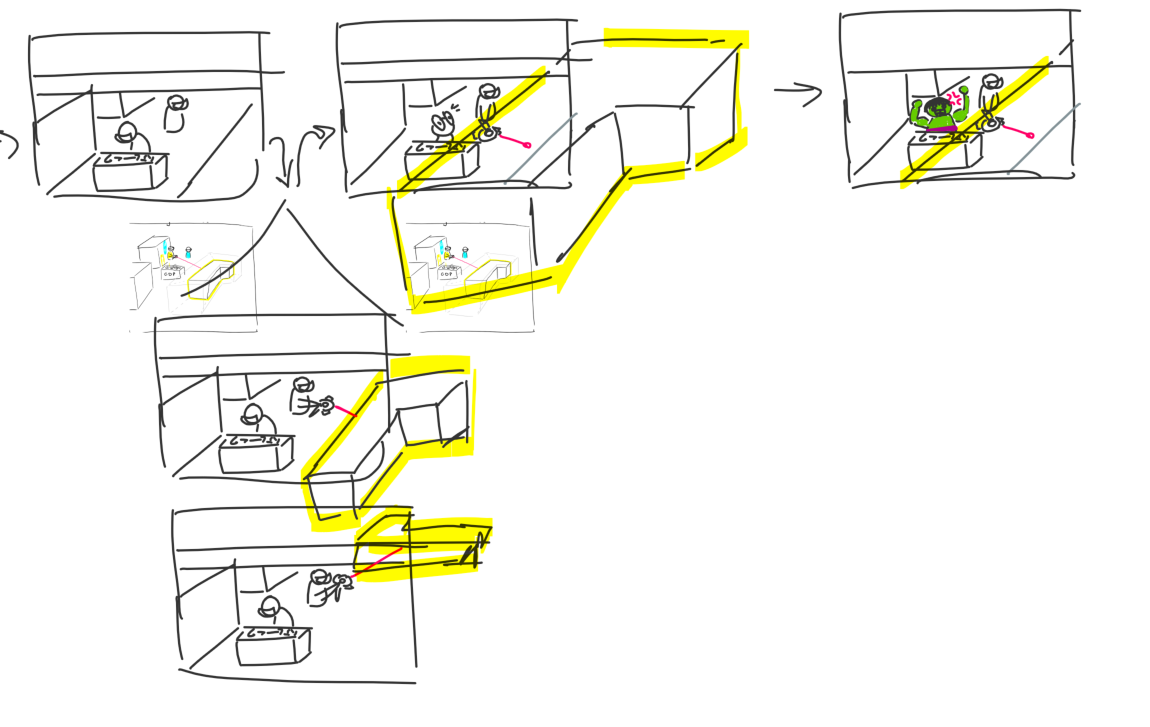
\includegraphics[width=0.7\linewidth]{figures/placeholders/A1_unaware_of_A2_actions}
	\caption{Collaborators unaware of each other's actions}
	\label{fig:a1unawareofa2actions}
\end{figure}

\paragraph{Buildings Popping Up} 
\label{buildingspoppingup}
The first prototype looked into how the participants' experience would be influenced, if a building suddenly appeared in-front of them, when they were occupied with their own task.

% Participants
3 participants (all male) were chosen among the members of the \gls{hci} group at the University of Otago. Two had prior experience in \gls{vr}, one had not.

% Procedure & Task
Participants were placed in the immersive \gls{vr} environment: a 3D model of the campus of the University of Otago. This was not a collaborative task, the participants were in the \gls{ve} alone. First, the the affordances of the environment were introduced (teleportation, walking and looking around), then participants were asked to navigate to the university clock tower. During this navigation task, a building would pop up in-front of them a couple of times at pseudo-random times (decided and initiated by the experimenter). After the completion of the experiment the participants were asked to describe the experience, especially the parts, where a building appeared in-front of them.

% Apparatus (i.e Unity, Resonance Audio, stereo headphones, Vive)
Unity3d and Oculus Rift \gls{hmd} with Touch Motion controllers were used in this experiment.

% Results
The participant with no prior experience in \gls{vr} described the experience as unexpected, but was also not sure, whether he caused it. The other two participants indicated that they were a bit stuttered by the experience, but in general, "didn't care much for it". Additionally, the participants described the experience as irritating, when the building continued to repeatedly appear after the first encounter.
% Limitations
% I do not check if anyone is concerned with the moving buildings when they get used to it.
% This doesn't matter tho, because according to the WA, people should know what the others are doing in the same environment.
% Discussion of the results?
%...


\paragraph{Moving Buildings}
Due to the results of the first experiment, the problem was regarded as worthwhile of further exploration. For the second proof of concept, a decision was made to come a bit closer to the initial motivation: buildings moving in \gls{ve}.
% Participants
4 new participant (all male) were chosen among the members of \gls{hci} group at the University of Otago, none took part in the previous experiment. Three had moderate experience with \gls{vr}, one had little.
% Procedure & Task
The environment affordances and the introduction remained the same. The task was extended, so that when participants find the clock tower, they were asked to assume their place at the viewing spot prepared for them (Fig. \ref{fig:prototype2viewvingspot}). At this point the participants were asked to observe the clock tower and tell the experimenter if anything seemed odd about it. Some elements of the tower were off axis (Fig. \ref{fig:prototype2clocktoweroddfeatures}), and this task was meant to lull participants' vigilance. As soon as participants started looking for any odd features, the movement of the clock tower towards the used with the speed of 200 units (meters) per second was initiated by the experimented. The approximate distance to from the viewing spot to the tower was 69 meters, the clock tower would stop 0.5 meters in-front of a participant. At this point the experiment would finish, and the participants would be asked about their experience.
\begin{figure}
	\centering
	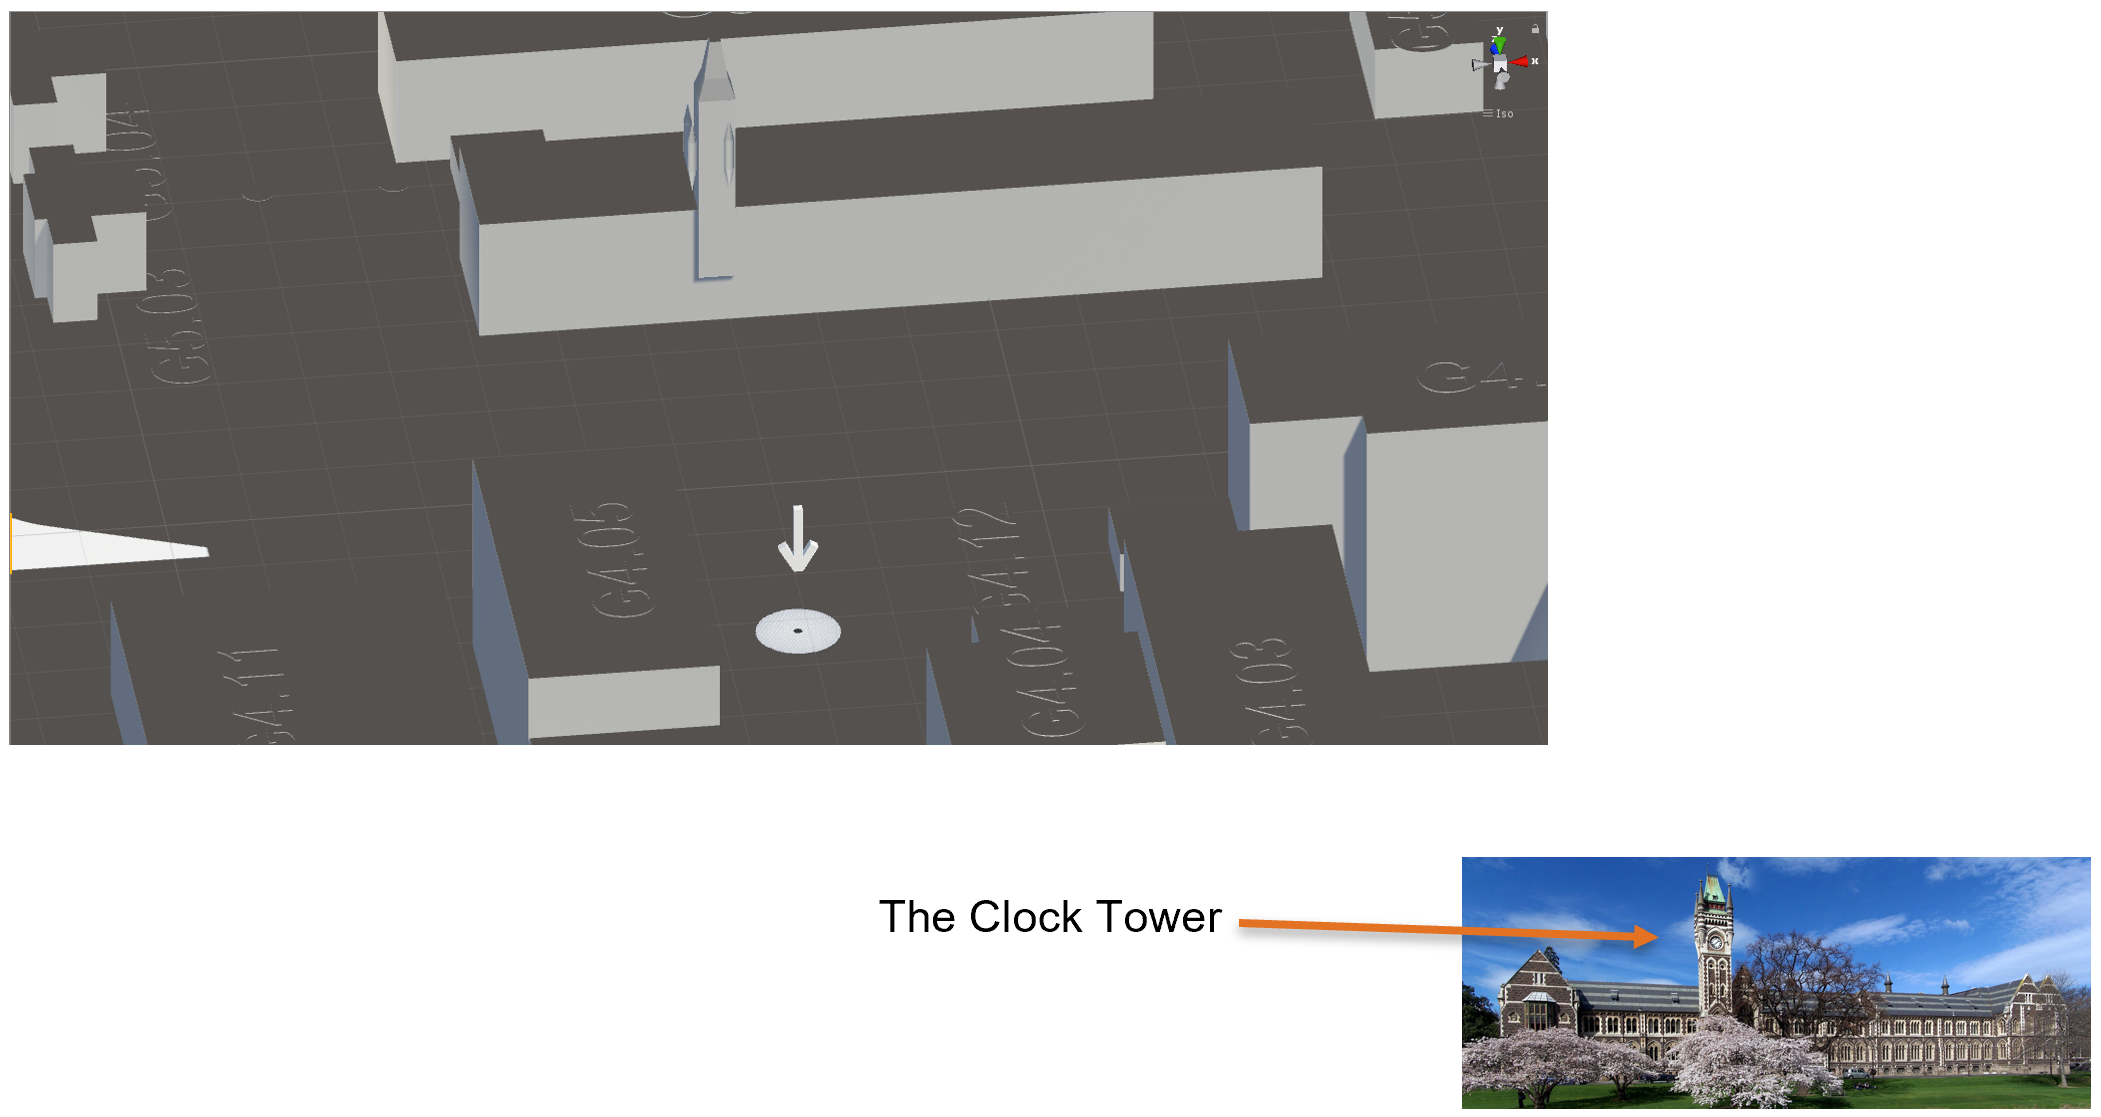
\includegraphics[width=0.7\linewidth]{figures/placeholders/prototype2_viewving_spot}
	\caption{The viewing spot in-front of the university clock tower}
	\label{fig:prototype2viewvingspot}
\end{figure}
\begin{figure}
	\centering
	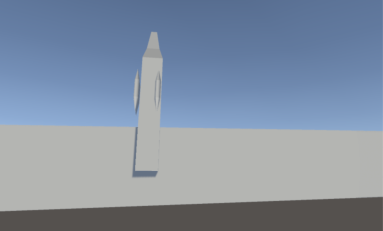
\includegraphics[width=0.7\linewidth]{figures/placeholders/prototype2_clocktower_odd_features}
	\caption{The odd features of the university clock tower model}
	\label{fig:prototype2clocktoweroddfeatures}
\end{figure}
% Apparatus
The same apparatus was used, as in the \nameref{buildingspoppingup} prototype.
% Results

% Limitations
\end{comment}


\section{Pilot Studies}
In preparation to the \nameref{final_study} study, two pilot studies were conducted: \nameref{study_one}, and \nameref{study_two}. This was done to study certain aspects of the final study separately, and make decisions, such as what sound type (earcons or auditory icons) to choose, and at what speed to translate the buildings.
















\subsection{Sound Speed and Type}
\label{study_one}
% Goal of the study
Some of the feedback from the initial prototypes indicates that the speed of the moving building was either too fast, or too slow. The goal of this study was to derive the speed participants felt would be appropriate to allow them to perform spatial judgments. Additionally, this pilot study was meant to help determine what type of auditory cues to use: earcons or auditory icons.

\paragraph{Participants}
Eight participants (7 men, 1 woman) were chosen among the members of the \gls{hci} group at the University of Otago, New Zealand. One had reported bad hearing, and one had a flu.  None of the participants had any architectural background, some were online gamers.
% TODO: figure out the age distribution

\paragraph{Procedure \& Task}
The study was carried out in a \gls{ve} that was specifically constructed for this purpose (see Fig. \ref{fig:clipimage001}). A participant was placed at the Center (C) of the environment, in which there was a real-sized building that could be translated by the experimenter from and to any of the predefined positions: Left Front (LF), Right Front (RF), Left Back (LB), Right Back (RB), Front (F), Back (B), Left (L), Right (R), C. When the building moved, a sound would emit from its position.

The purpose the whole research and this study was explained to the participants. They were placed at the center of the scene (C) with the building placed in front of them, and asked to preserve the orientation of the chair they were seated upon, but were also told that they were allowed to move their head.

Participants were put through a tutorial to build a correlation between the visually perceived movements of the building and the emitted sound: the building was translated along the major directions (C-F, C-L, L-R, L-C, C-B), and then additionally between randomly selected positions from the predefined set (Fig. \ref{fig:pilot1predefinedtutorialtranslations}).

At the start of the actual experiment, participants were asked to close their eyes and guess the path that the building traversed. It was silently positioned at a randomly selected position and then translated with auditory cues to a newly selected random position (see Fig. \ref{fig:arbitrary_translation}). This was repeated 5 to 10 times for each of 6 type of sound-speed combinations.

After going through all the sound types and speeds, participants were asked for their honest opinion, as to which sound was the best, and what speed was the most appropriate.

\begin{figure}
	\centering
	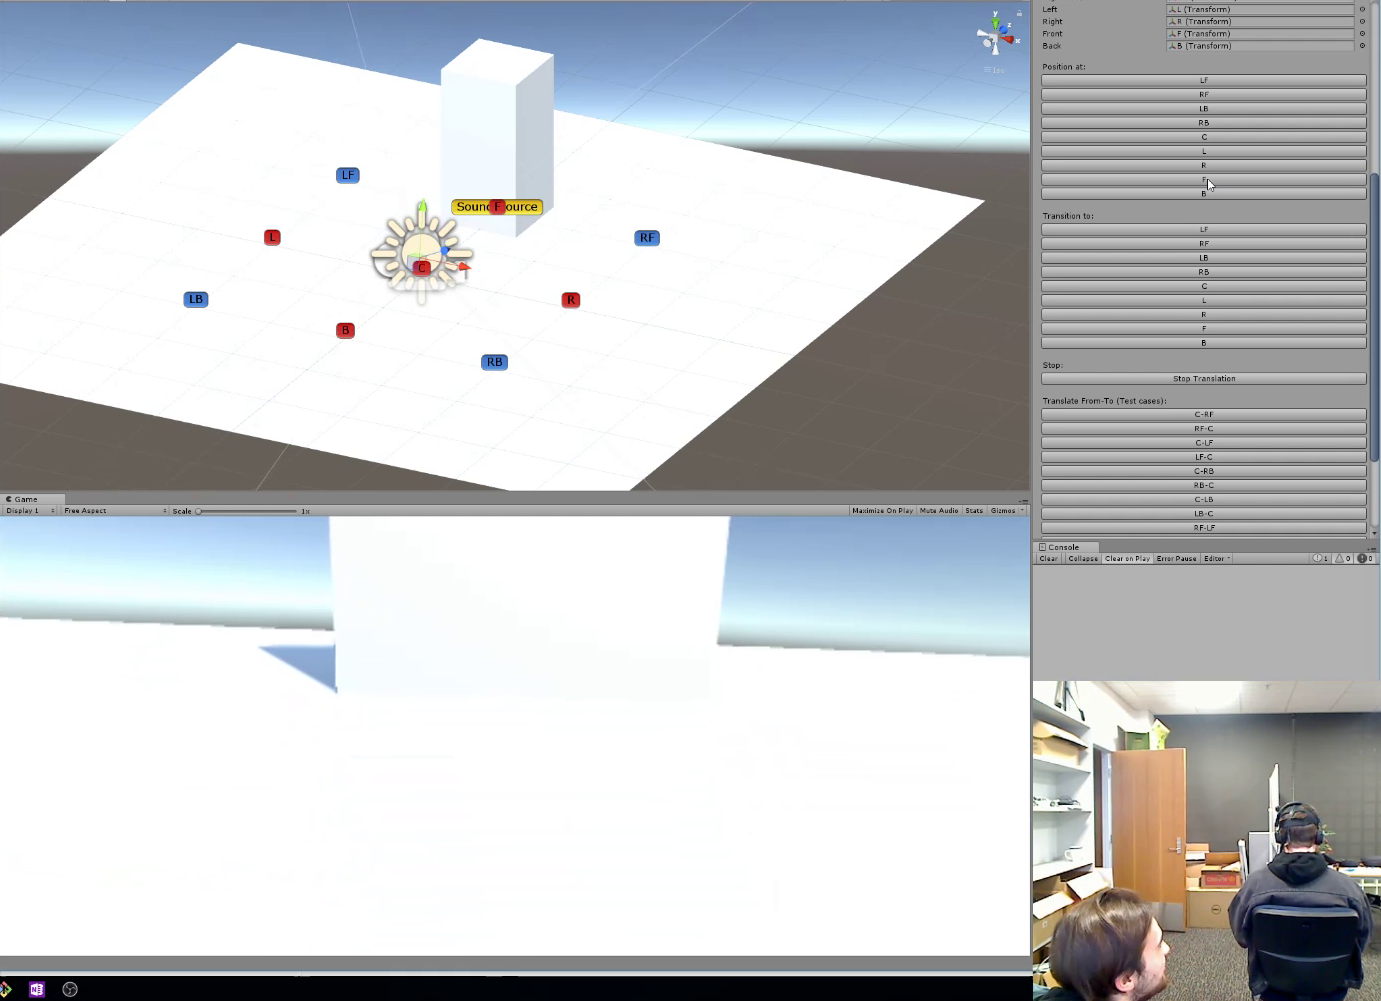
\includegraphics[width=0.7\linewidth]{figures/placeholders/pilot1_experiment_setup.png}
	\caption{Experiment setup}
	\label{fig:clipimage001}
\end{figure}

\begin{figure}
	\centering
	\subfloat[Predefined translation paths]{
		\label{fig:pilot1predefinedtutorialtranslations}
		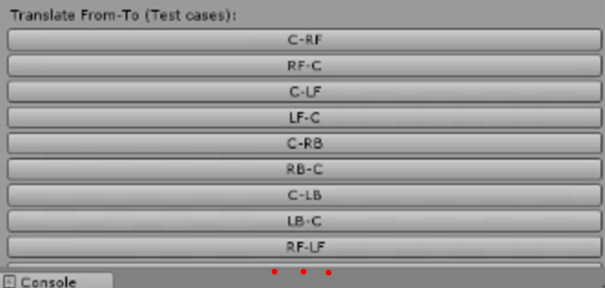
\includegraphics[width=0.3\linewidth]{figures/placeholders/pilot1_predefined_tutorial_translations}
	} %

	\subfloat[Arbitrary translations]{
		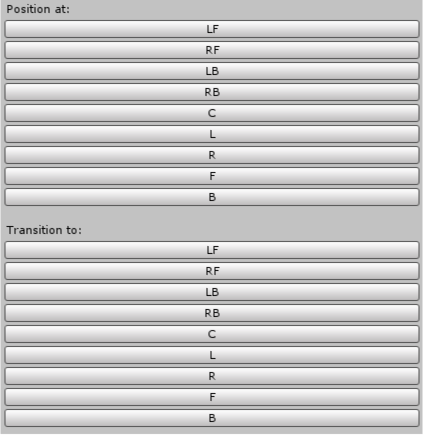
\includegraphics[width=0.3\linewidth]{figures/pilot1_control_panel}
		\label{fig:arbitrary_translation}
	}
	
	\caption{Control panels}
	\label{fig:pilot1controlpanel}
\end{figure}


\paragraph{Apparatus}
% Apparatus (i.e Unity, Resonance Audio, stereo headphones, Vive)
Experiment was implemented with the help of Unity3d  2018.1.5f1 and Resonance Audio SDK for Unity, version 1.2.1 with sound occlusion turned off. For the hardware, HTC Vive \gls{vr} headset, along with on-ear stereo headphones, and a Windows 10 PC.
Audacity 2.2.2 was used prior to the experiments to: mixdown stereo sounds to mono, make audio tracks seamless, and increase the volume.

% Study Factors and Conditions: what my factors are, conditions == independent variables' values
\paragraph{Study design}
The study followed the repeated measures design with 2 independent variables: translation speed and different types of auditory cues.

Three different translation speeds were tested: \textit{slow} - 20, \textit{medium }- 40, and \textit{fast }- 60 meters per second (m/s). Sound properties (i.e. pitch, playbackspeed) stayed constant throughout the different speeds.

Two different types of the auditory cues were tested: earcons and auditory icons. A full volume 100 Hz sine wave in mono was used for an earcon (Type: Wave (.wav), Samplerate: 44100.0 Hz, Bitdepth: 16bit, Source: https://freesound.org/people/klangfabrik/sounds/28638/, Fig. \ref{fig:pilot1sinewaveedit}). As an auditory icon a mono sound mimicking moving concrete block with sound amplitude extrema reaching full volume was used (Type: Wave (.wav), Samplerate: 48000.0 Hz, Bitdepth: 16 bit, Source: https://freesound.org/people/FreqMan/sounds/25846/, Fig. \ref{fig:pilot1concreteonconcretesoundedit}).
The type of sound played first was rotated for the participants, so that 4 of them heard the auditory icon first, and the other 4 - the earcon.

\begin{figure}
	\centering
	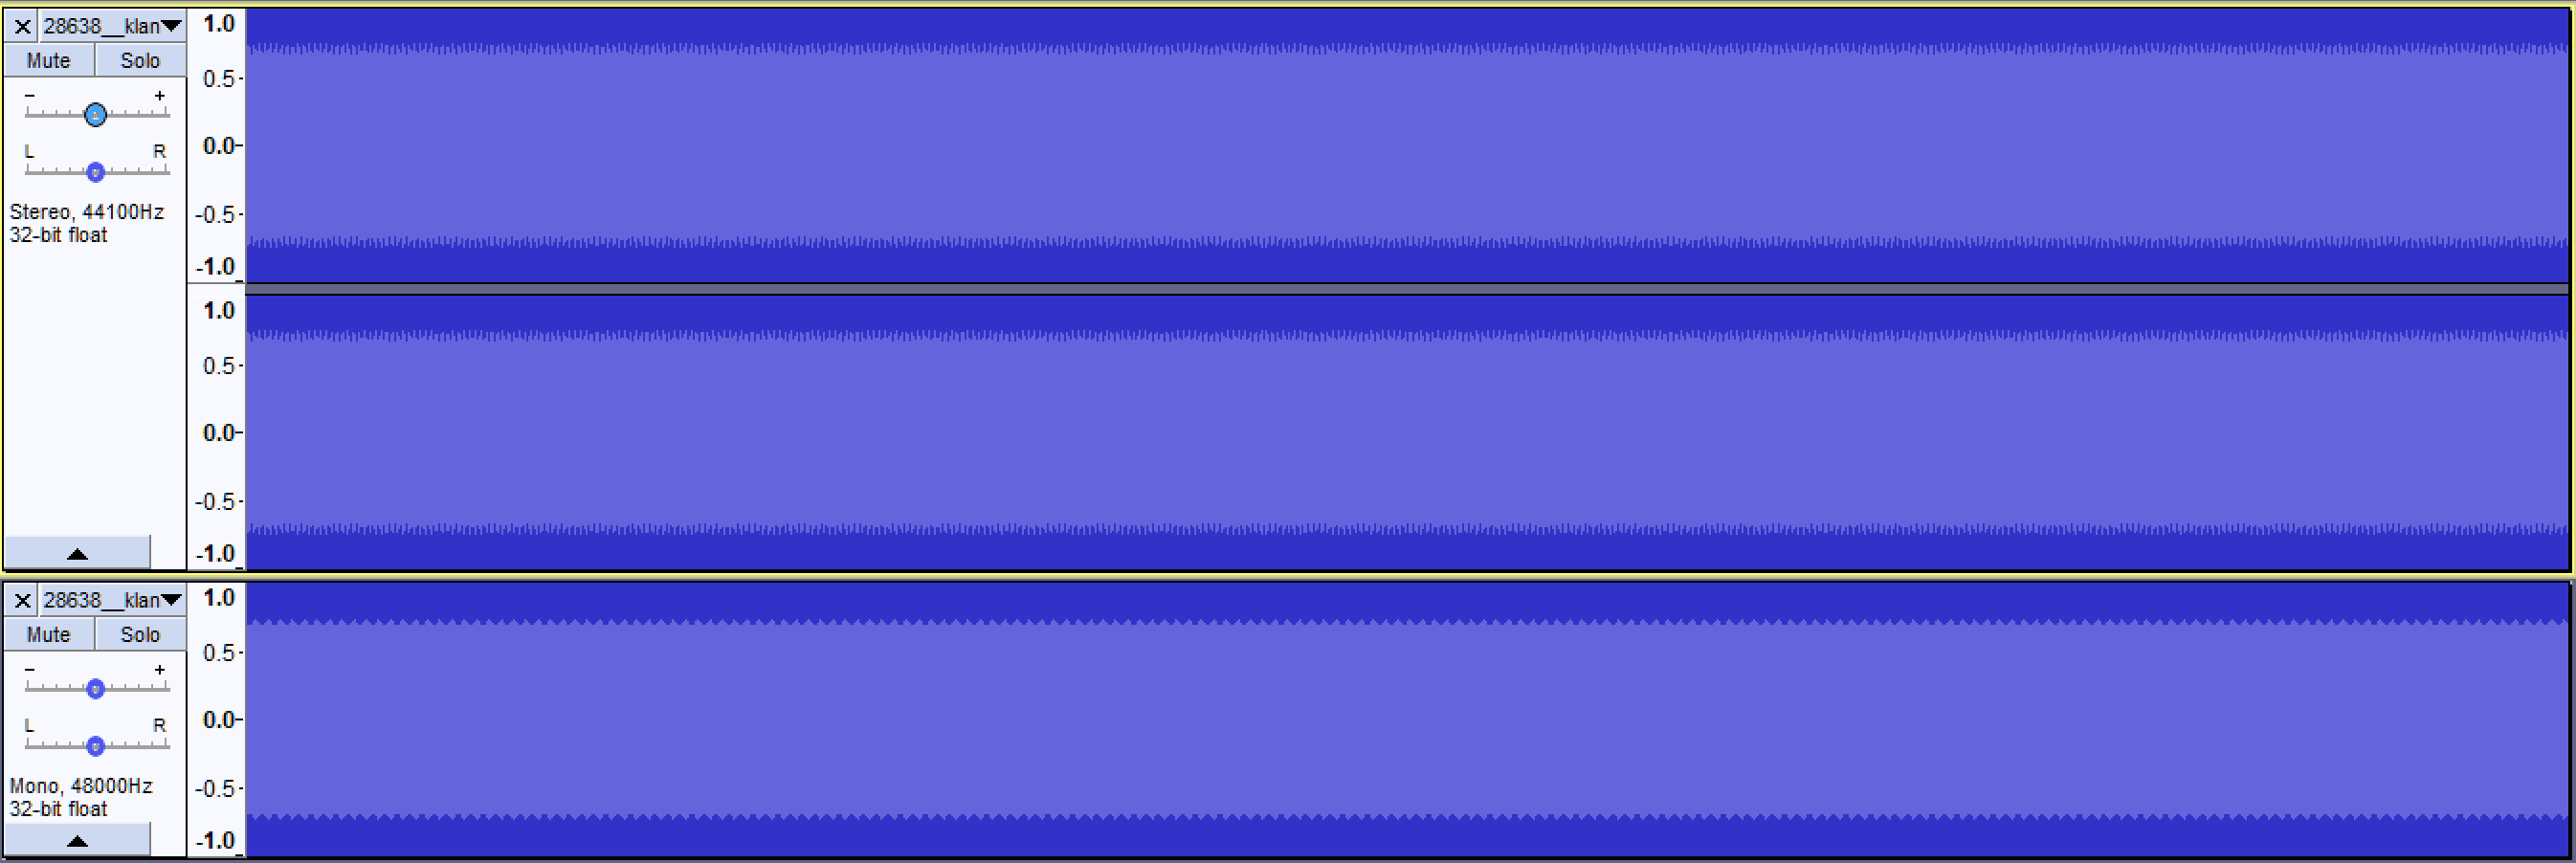
\includegraphics[width=0.7\linewidth]{figures/pilot1_sinewave_edit}
	\caption{Sine wave earcon before (top) and after (bottom) mixdown: stereo to mono}
	\label{fig:pilot1sinewaveedit}
\end{figure}

\begin{figure}
	\centering
	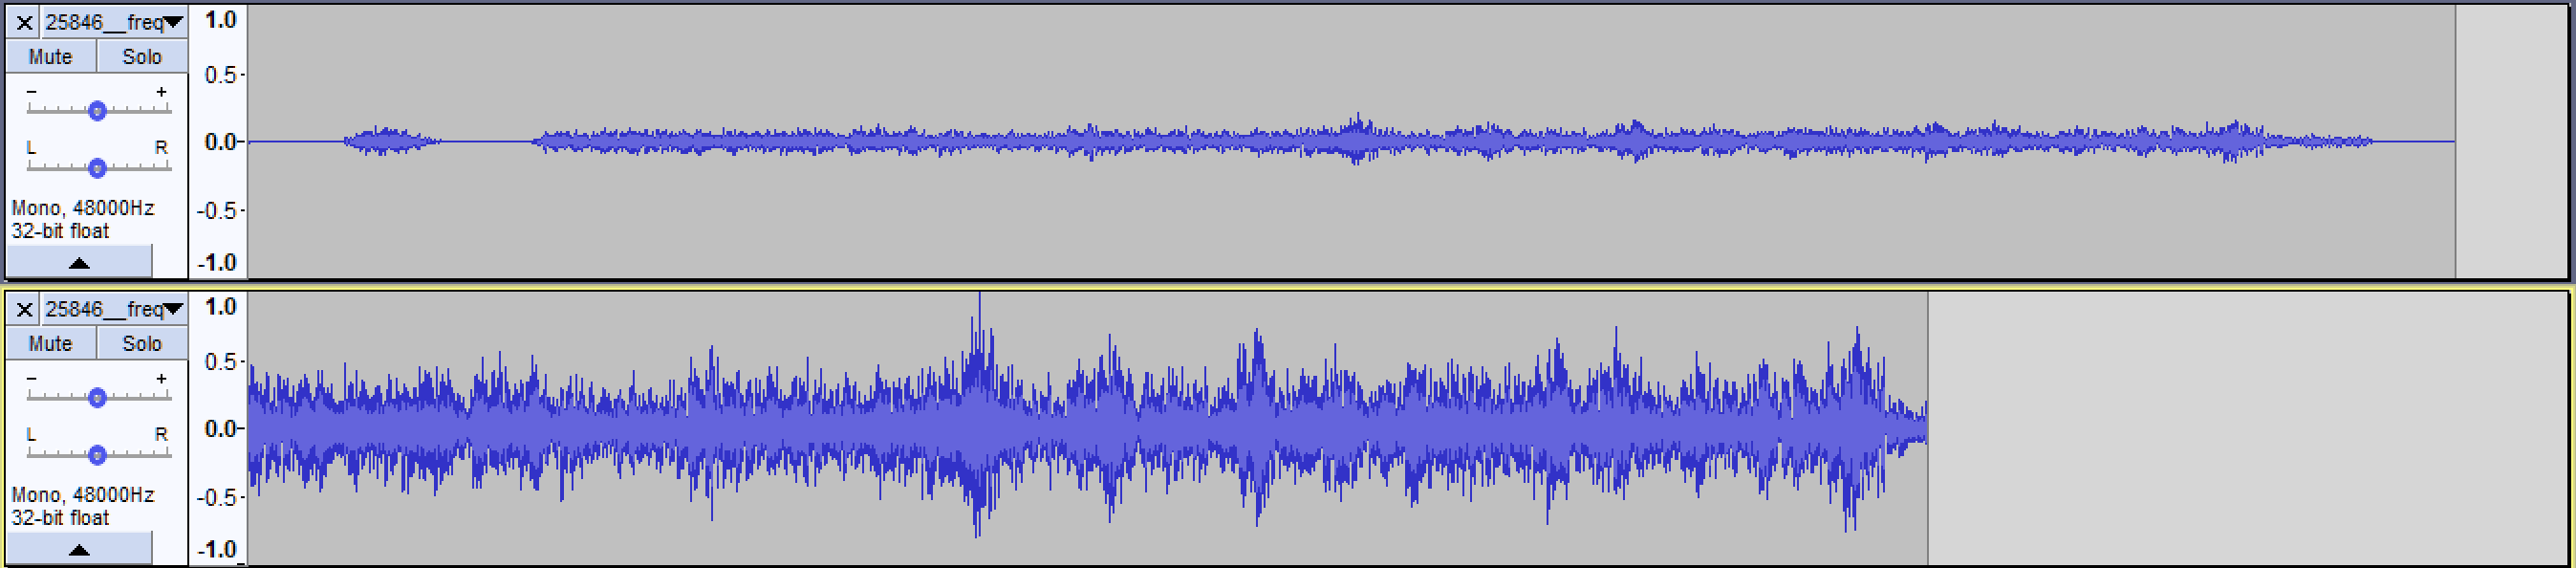
\includegraphics[width=0.7\linewidth]{figures/pilot1_concrete_on_concrete_sound_edit}
	\caption{Concrete sliding on concrete auditory icon before (top) and after (bottom) amplification, and crop}
	\label{fig:pilot1concreteonconcretesoundedit}
\end{figure}

Translations were pseudo-randomized across participants, their selection was made with some degree of bias towards longer translation paths, so that users have more time to analyze the sound and guess (i.e. the path from RB to LB would be longer, than just RB to B). Different translation paths can be seen in Fig. \ref{fig:pilot1translationpaths}.

Distances between the fixed translation end-points remained the same throughout the experiment: 20 Unity3d units (meters) between C-F, C-L, C-R, C-B, L-LB, and so on.

\paragraph{Results}
\textit{Preferred sound} 6 out of 8 participants preferred the concrete sound to the sine wave, 1 was indifferent as long as the speed was slow, and 1 preferred the sine wave.

\textit{Preferred speed} The speed preference can be seen in the Table \ref{table:pilot1_results}.

\begin{figure}
	\centering
	
	\subfloat[Top-down view of the scene]{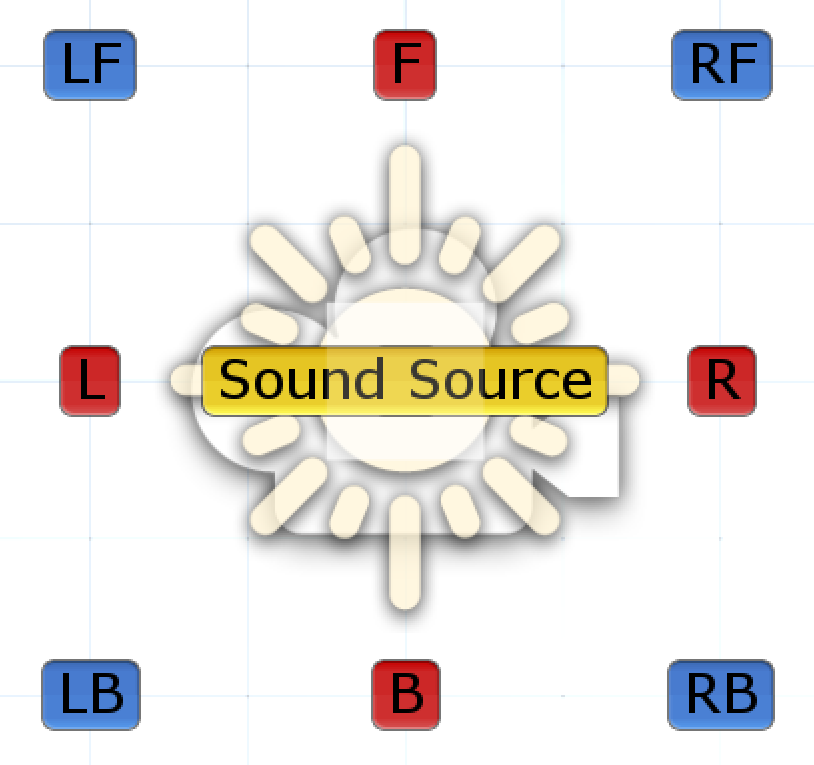
\includegraphics[scale=.4]{figures/pilot1_top_down_scene_view.png}}%
	\subfloat[Major translation paths]{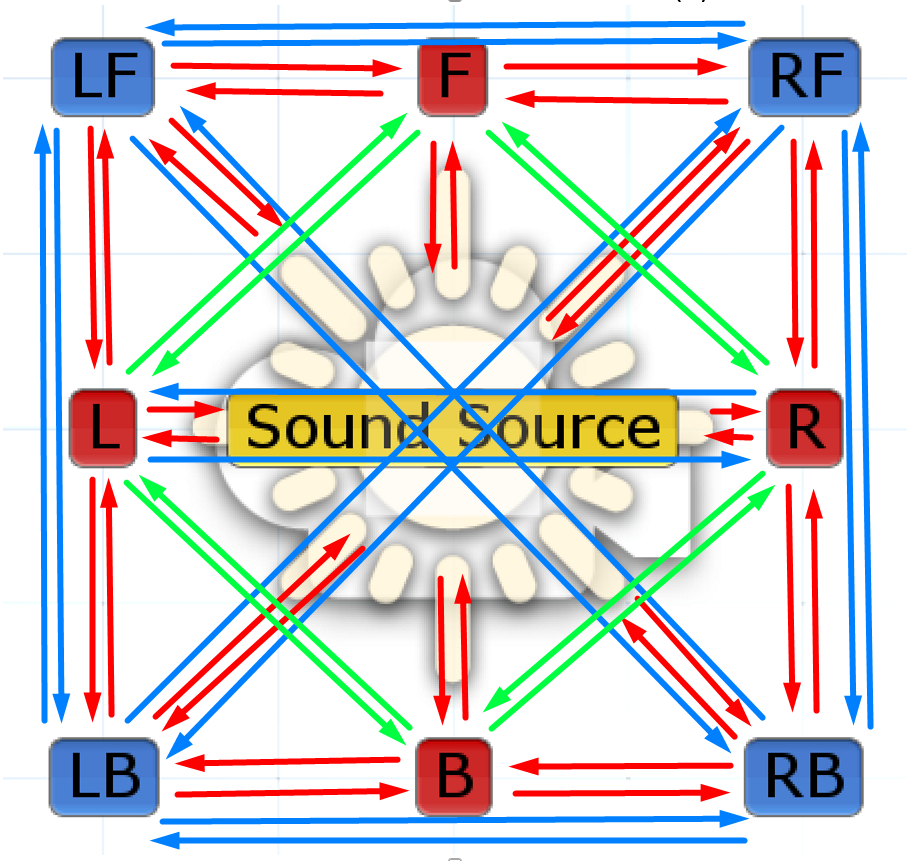
\includegraphics[scale=.4]{figures/pilot1_top_down_scene_view&major_tranlsation_paths.png}}%
	\subfloat[All translation paths]{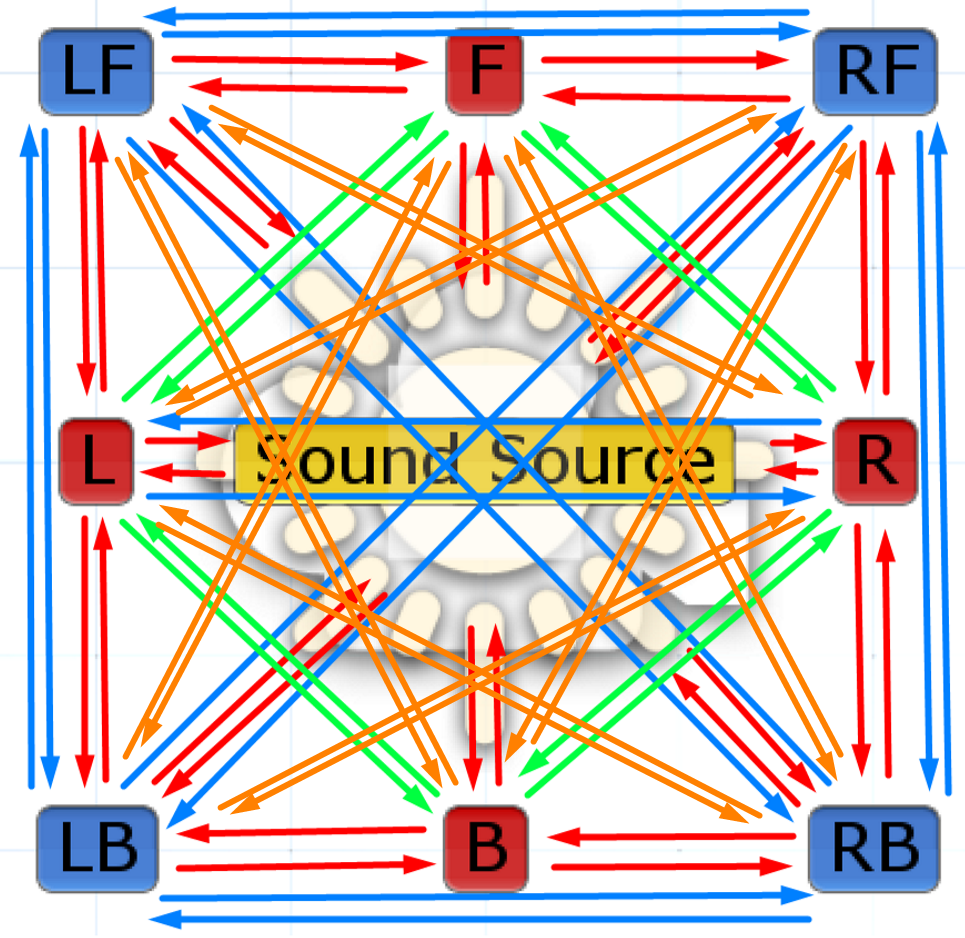
\includegraphics[scale=.4]{figures/pilot1_top_down_scene_view&all_possible_translation_paths.png}}
	
	\caption{Possible translation end-points and paths}
	\label{fig:pilot1translationpaths}
\end{figure}


\begin{table}[h]
	\label{table:pilot1_results}
	\caption{Experiment data}
	
	\begin{tabular}{|l|l|l|l|}
		\hline
		\textbf{Participant} & \textbf{First sound played} & \textbf{Preferred sound} & \textbf{Preferred speed}                        \\ \hline
		1                    & Concrete                    & Concrete                 & Medium                                          \\ \hline
		2                    & Concrete                    & Concrete                 & Slowest, then medium                            \\ \hline
		3                    & Sine wave                   & Concrete                 & Medium                                          \\ \hline
		4                    & Sine wave                   & Concrete                 & First two -fine (fastest one - a bit too fast)  \\ \hline
		5                    & Concrete                    & Either                   & Slowest                                         \\ \hline
		6                    & Sine wave                   & Sine wave                & Fast (speed didn't affect it too much)          \\ \hline
		7                    & Concrete                    & Concrete                 & Between slow and medium                         \\ \hline
		8                    & Sine wave                   & Concrete                 & First two - fine (fastest one - a bit too fast) \\ \hline
	\end{tabular}
\end{table}

\paragraph{Discussion}
If we visualize the participants' preferences, and take the smallest common area, where they overlap, analysis shows that participants preferred the speed somewhere close to 40 m/s, but between 20 and 40 (Fig. \ref{fig:pilot1resultsanalysis})

The preferred (concrete on concrete) sound, which was described by one participant as "dry and dull", has a distinct timbre, which is made of different harmonics and halftones. The sine wave, on the other hand, has only 1 fundamental frequency, which might make memorizing and spatial differentiation harder. Additionally, this frequency would most likely get cut of by the audio SDK, if occlusion effect was to be used.

\begin{figure}	
	\centering
	
	\subfloat["Medium"]{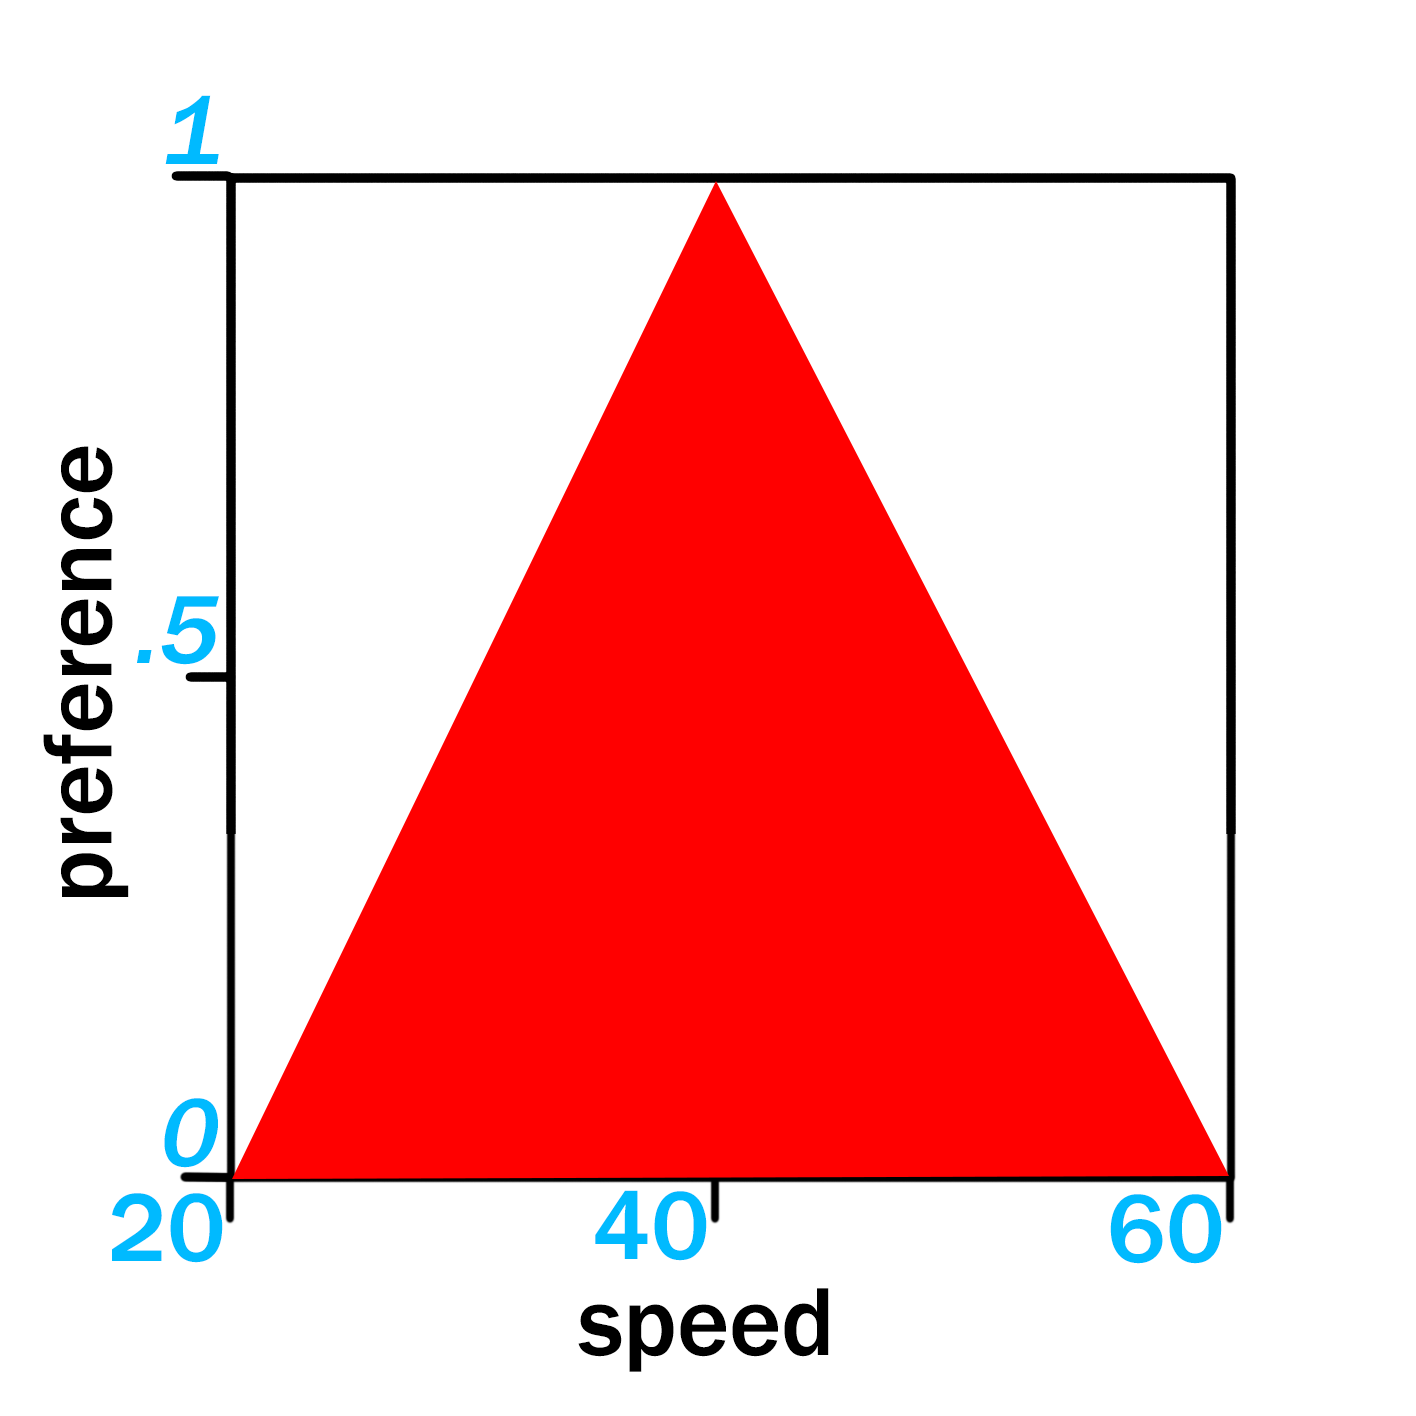
\includegraphics[scale=.075]{figures/pilot1/results/speed_fuzzy_preference_medium.png}}%
	\subfloat["Slowest, then medium"]{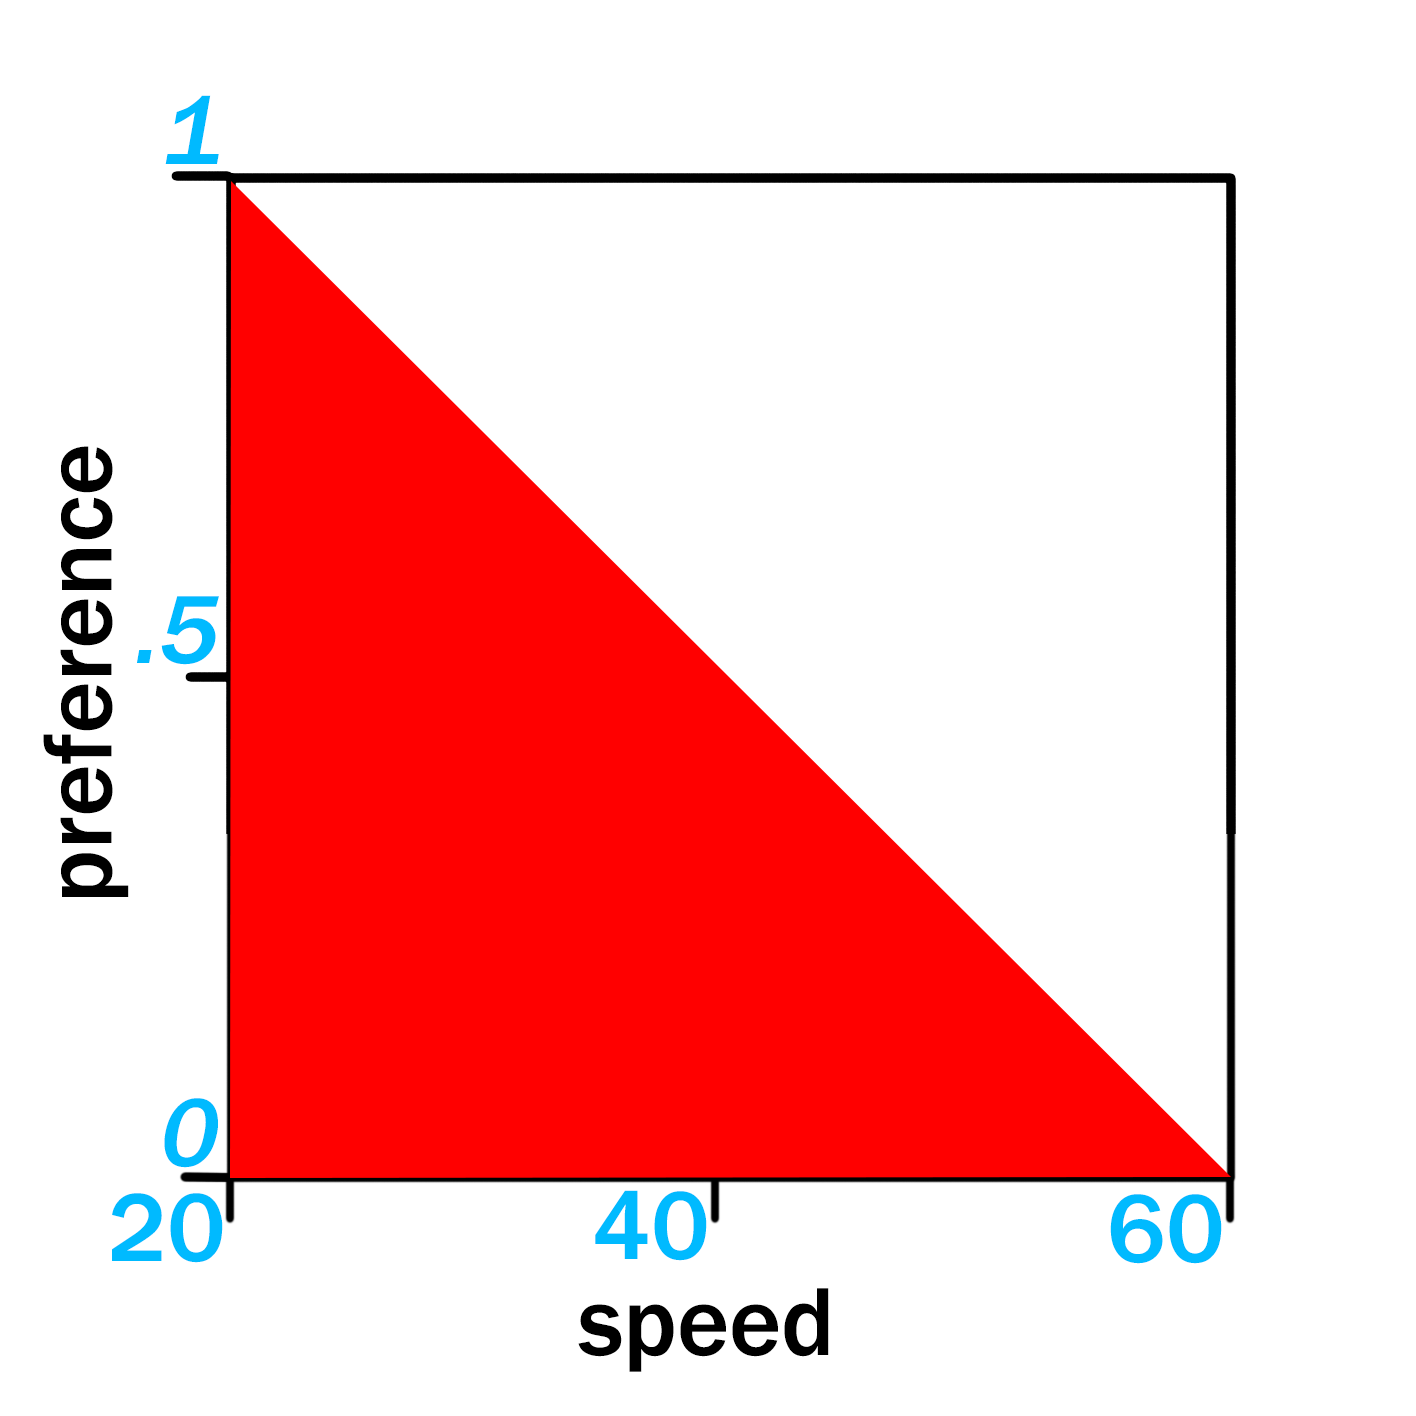
\includegraphics[scale=.075]{figures/pilot1/results/speed_fuzzy_preference_slowest_then_medium.png}}%
	\subfloat["First two - fine..."]{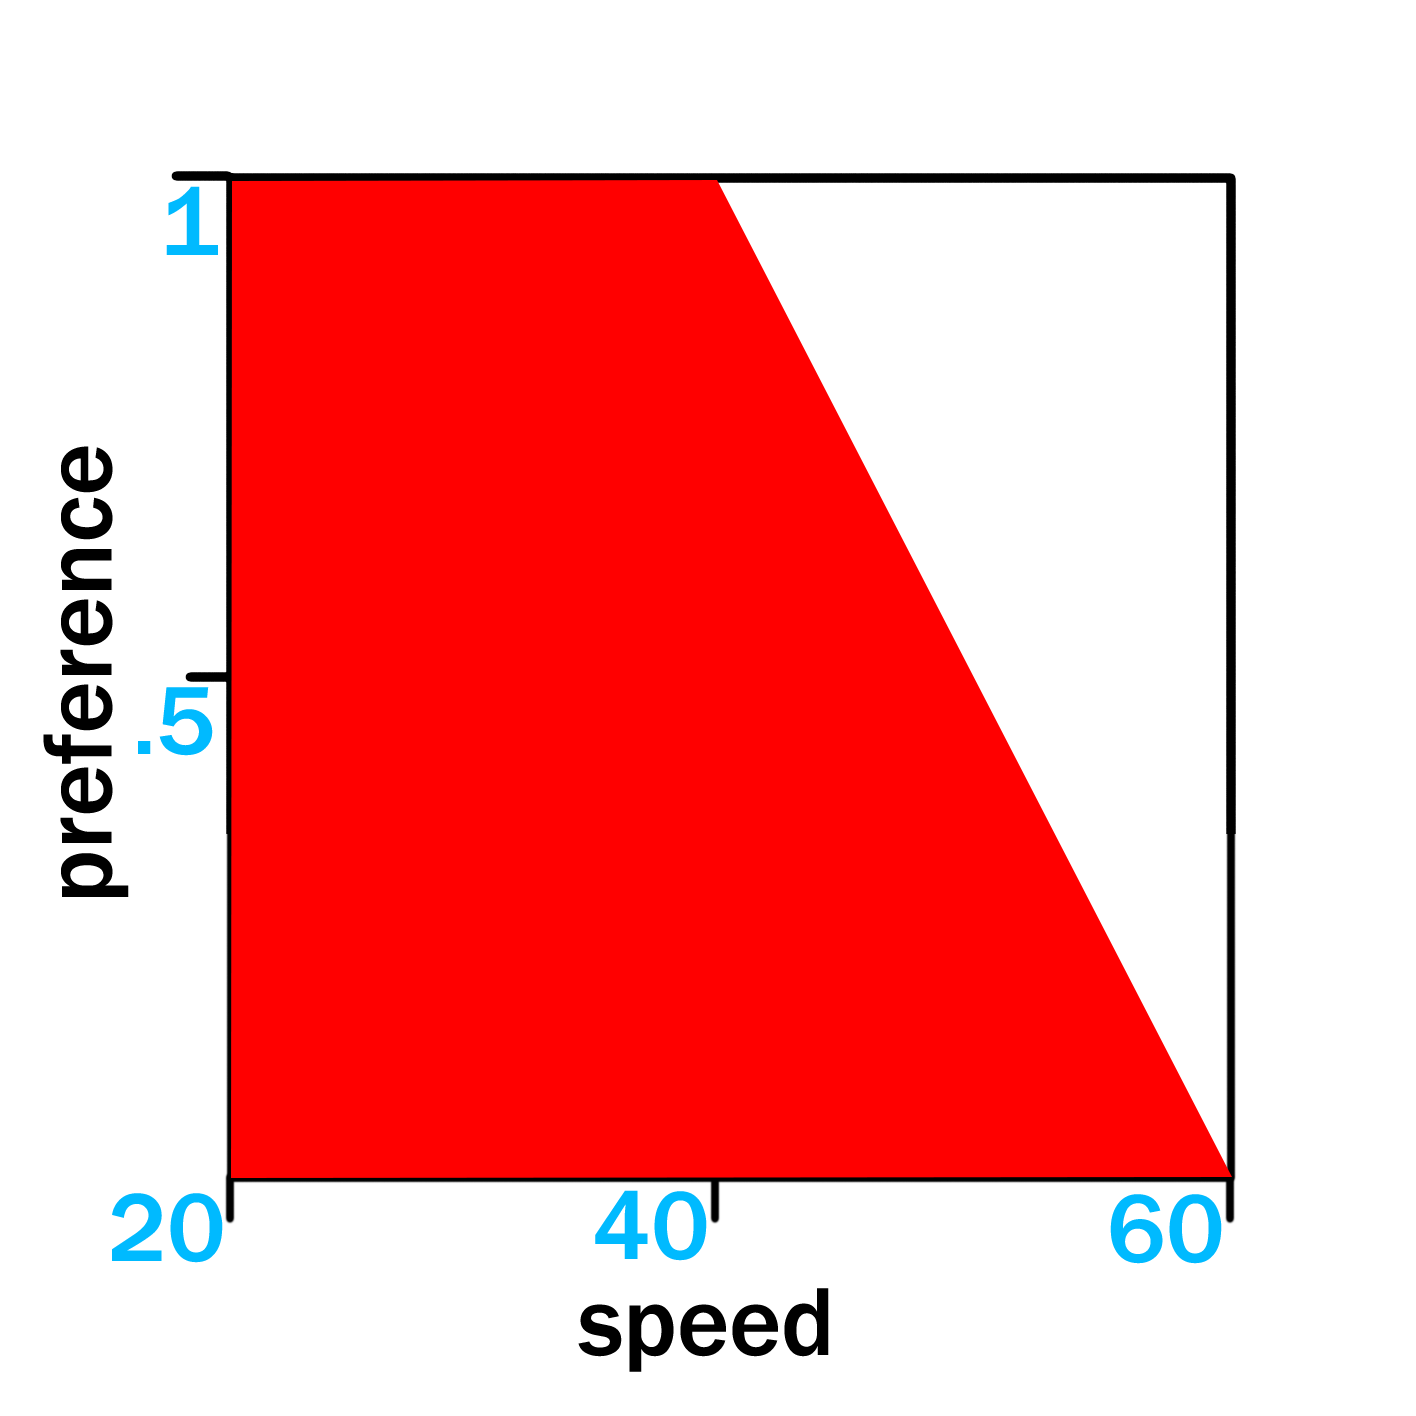
\includegraphics[scale=.075]{figures/pilot1/results/speed_fuzzy_preference_first_two_fine.png}}%
	\subfloat["Slowest"]{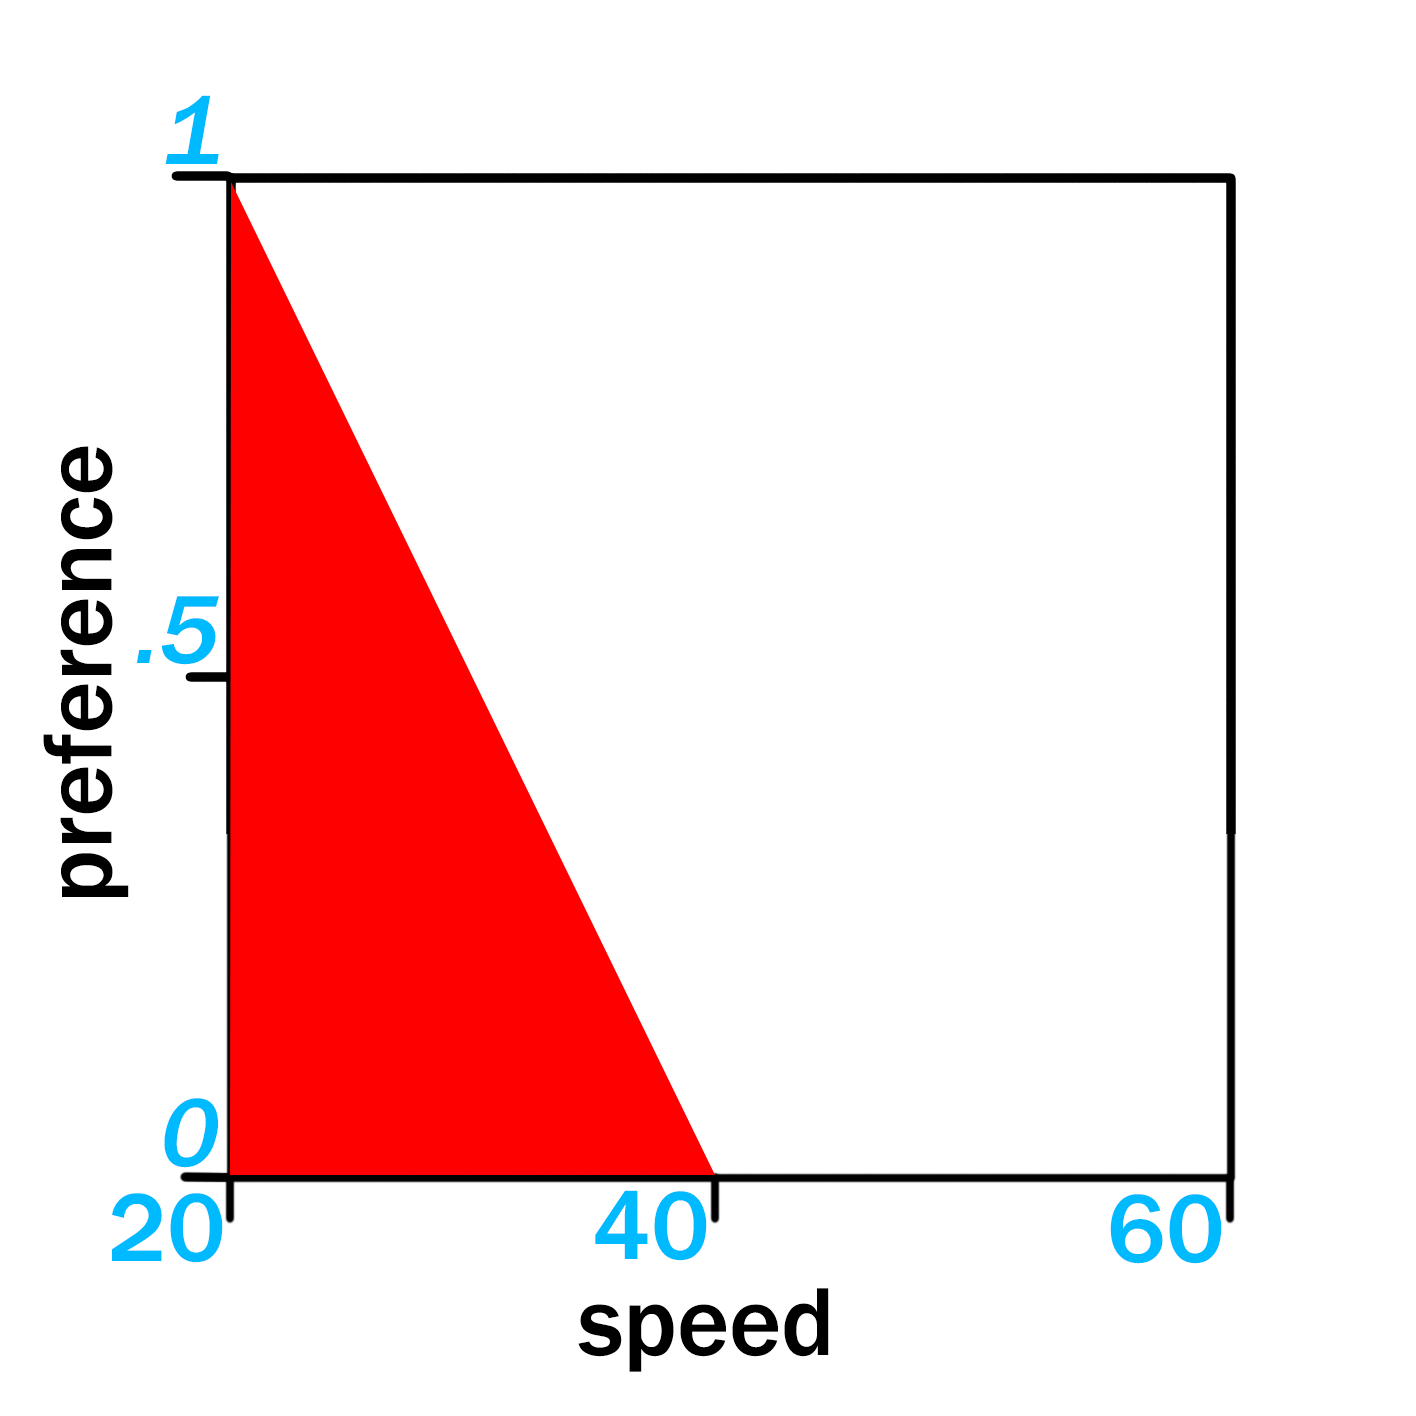
\includegraphics[scale=.075]{figures/pilot1/results/speed_fuzzy_preference_slowest.png}}
	
	\par\medskip
	\subfloat["Fast..."]{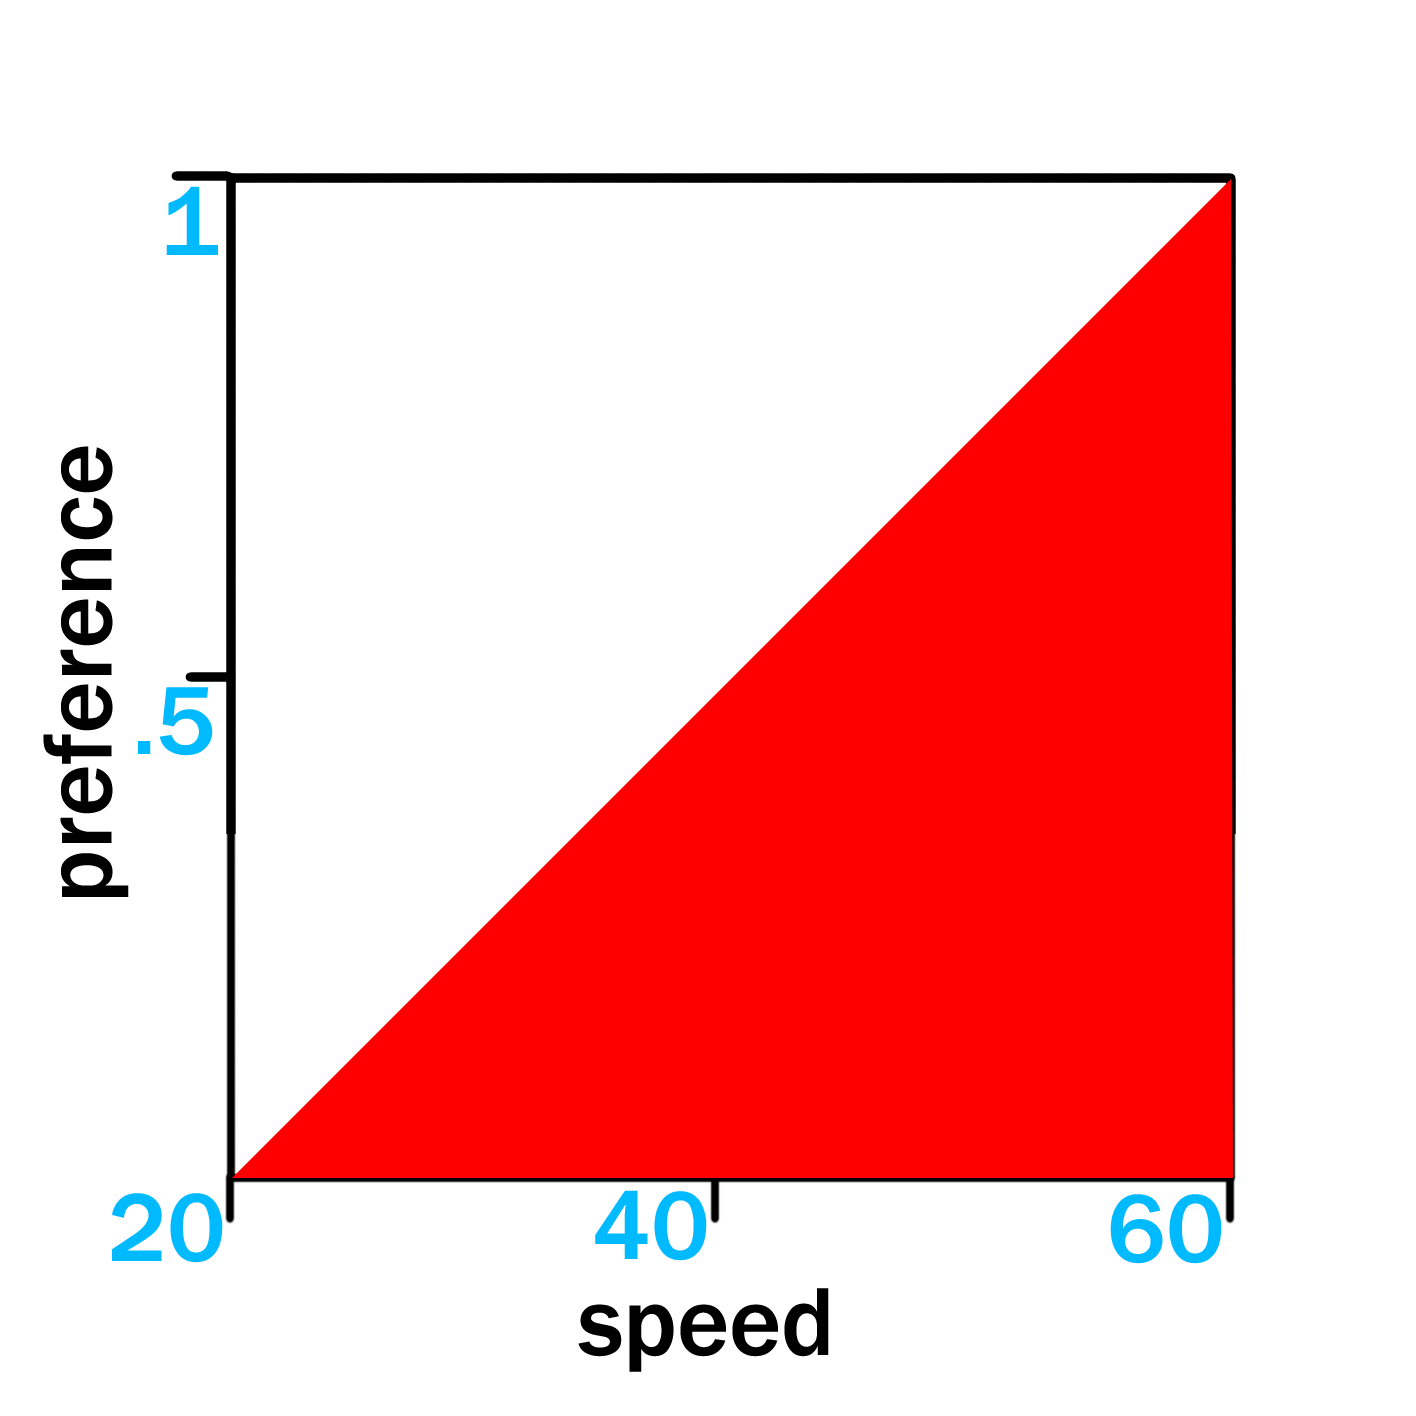
\includegraphics[scale=.075]{figures/pilot1/results/speed_fuzzy_preference_fast.png}}%
	\subfloat["Between slow and medium"]{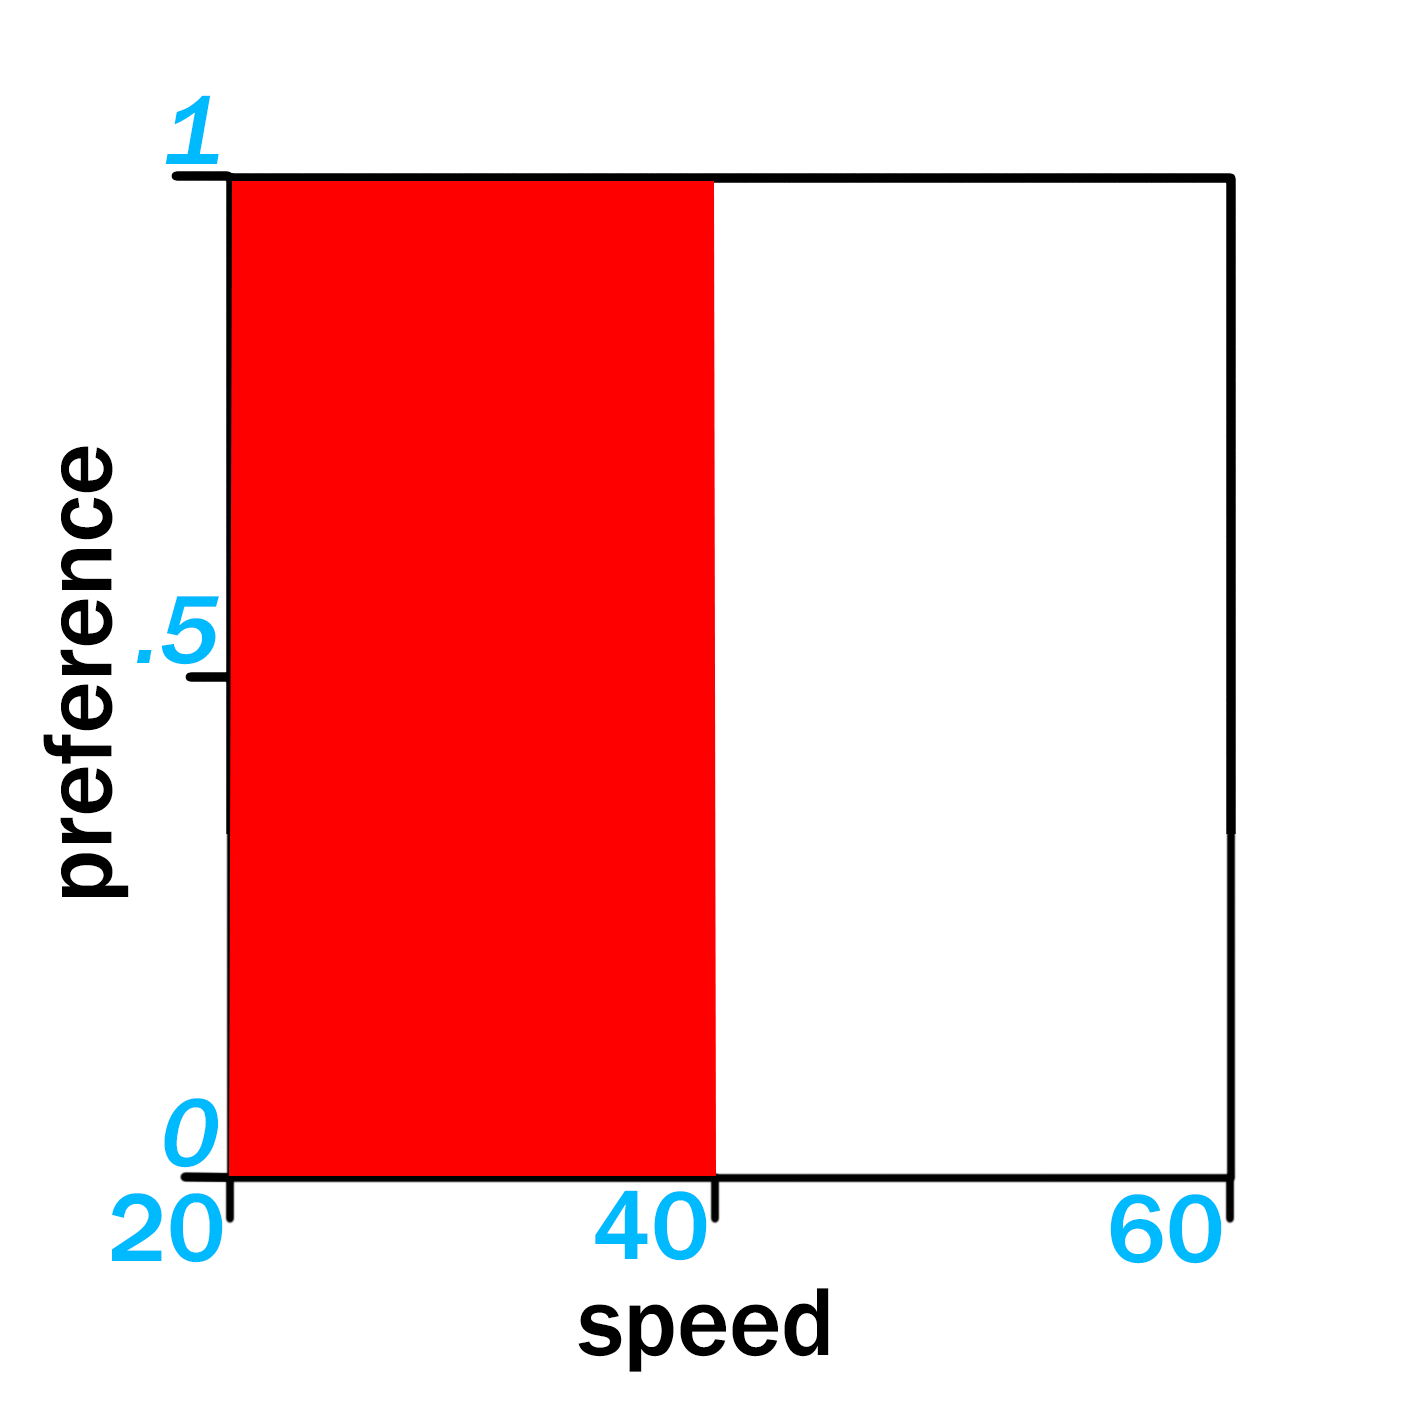
\includegraphics[scale=.075]{figures/pilot1/results/speed_fuzzy_preference_between_medium_and_slow.png}}%
	\subfloat[Answers combined with 12\% opacity each]{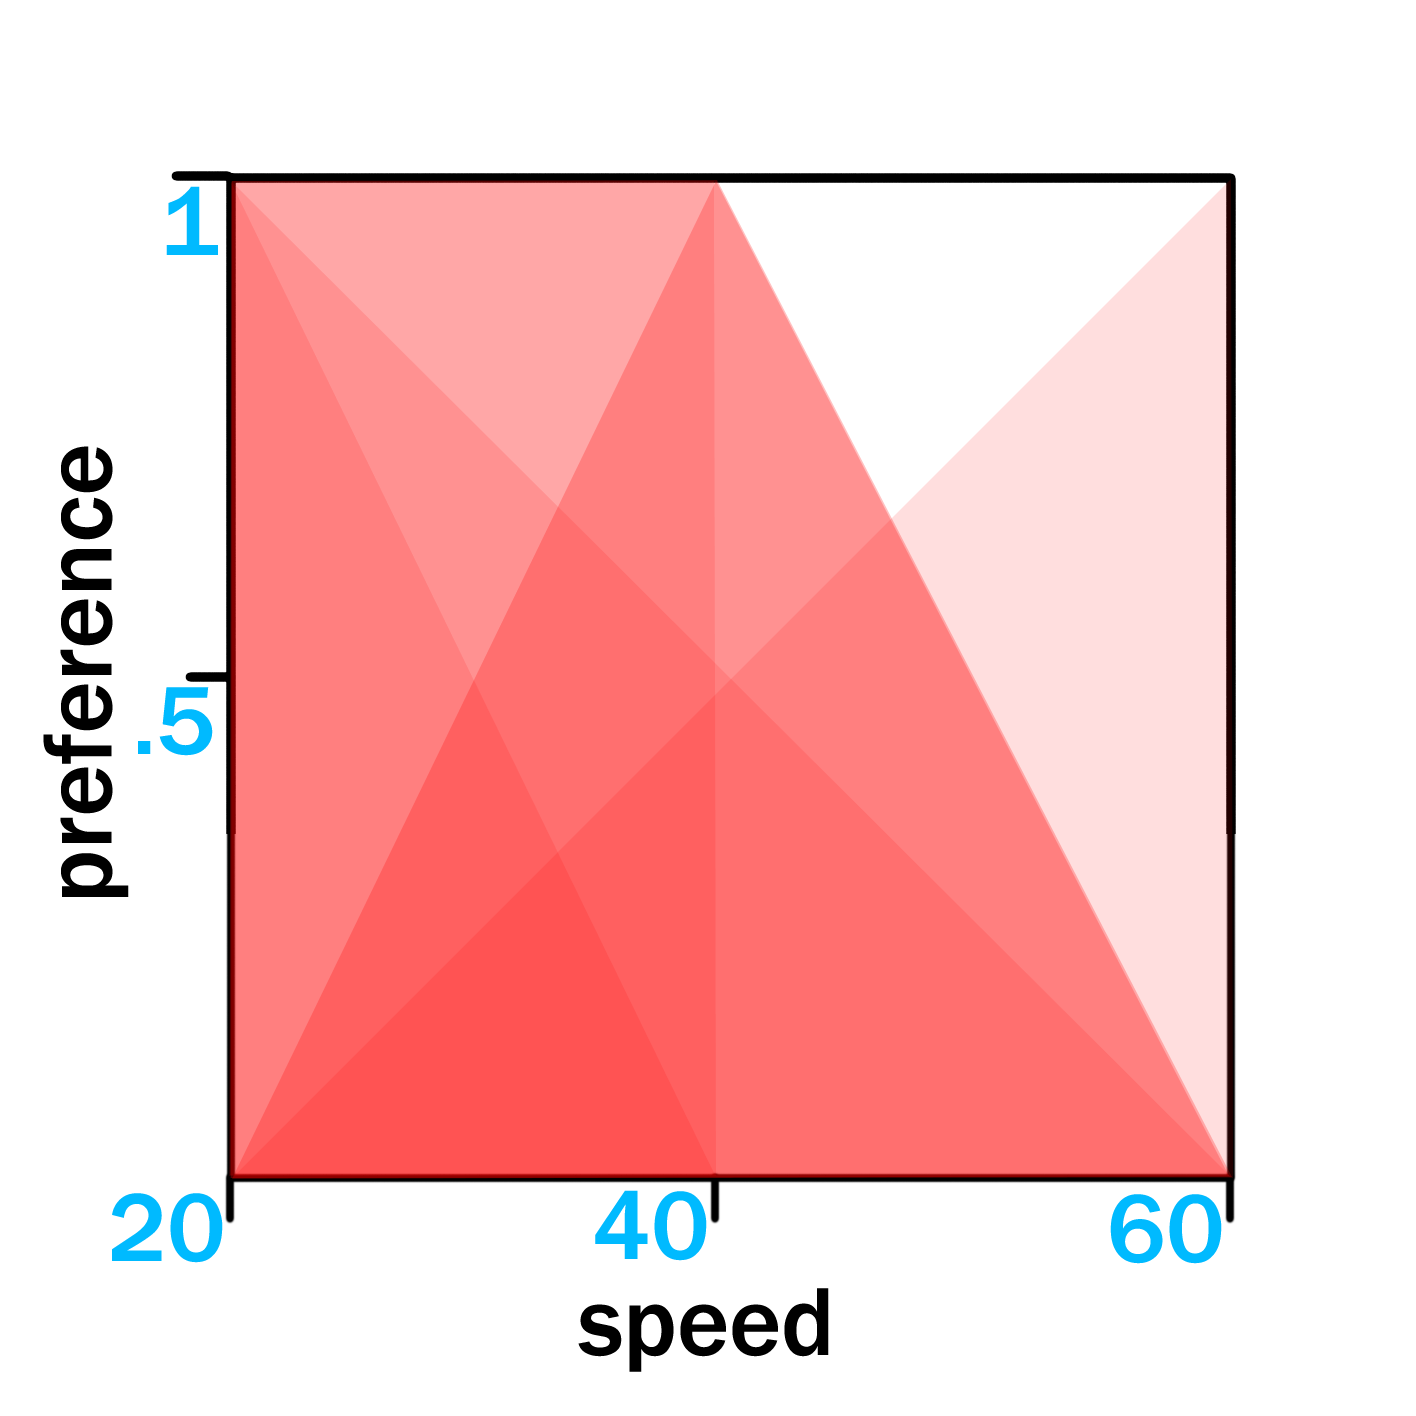
\includegraphics[scale=.075]{figures/pilot1/results/speed_fuzzy_preference_result_no_highlight.png}}	
	
	\par\medskip
	\subfloat[Preferred speed according to analysis]{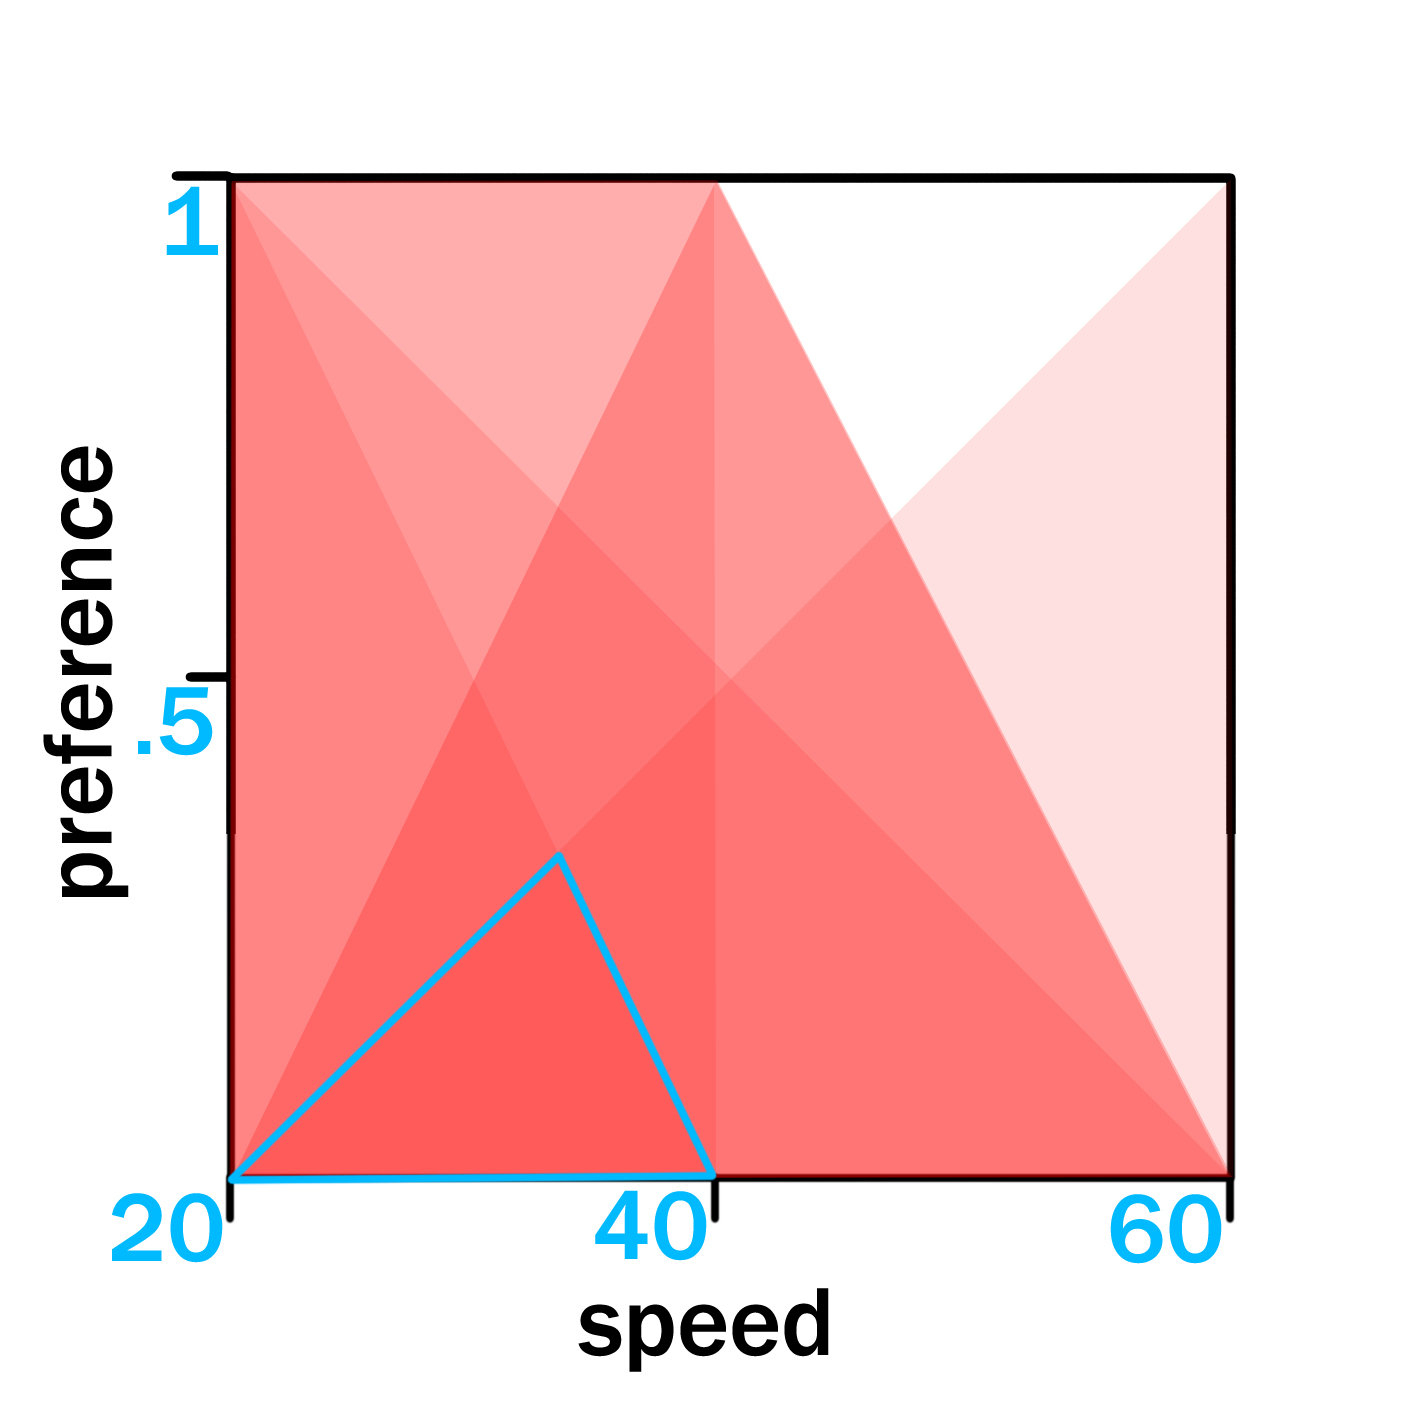
\includegraphics[scale=.15]{figures/pilot1/results/speed_fuzzy_preference_result.png}}
	
	\caption{Visual analysis of results, pilot 1}
	\label{fig:pilot1resultsanalysis}
\end{figure}

\subparagraph{Limitations} 
\textit{Auditory variation} Only 2 different types of auditory cues were used in this study to indicate the translation of the building. Different sounds might need to be tested to take advantage of different sound properties on the ability to interpret the spatial sound. 

\textit{Front-to-back confusion} One of the major observation was the inability of participants to differentiate between translations happening in the back and in the front. For example, the translation from RF to LF was mistakenly indicated as RB to LB.
%The confusion between front to back has to been pointed out to might have something to do with the sound reproduction in stereo headphones

\textit{Visualization} As it was a preparatory study, the participants were simply asked to close their eyes when guessing the path of the building. Besides the obvious drawback of such approach, participants reported that it is possible to predict the path by relying on the change in brightness, which is perceivable even with the eyes closed, when the building is passing by.

\textit{False negatives} Some users, who gave answers that were close to correct (i.e. the building was reported to move from R to LB, when in reality it moved from RB to LB), indicated that they were not aware that the building can move along such a path. 
% TODO: do I add the next sentence or do I put it in the next pilot?
%This means that users have to be thoroughly instructed on all the possible translation paths before the start of the guessing tests to avoid false negatives.












\subsection{Spatial Judgment}
\label{study_two}
%Goal
The goal of the second pilot study was to see how much information can sound convey about the buildings moving in the environment, and how much of a problem the front-to-back confusion actually causes. Additional motivation was to pilot the way for participants to point out the changes to the environment, which would be needed in the final study to infer the \gls{wa} index. 

\paragraph{Participants}
Thirteen participants (9 men and 4 women; mean 29.4, std. 10.7) were selected from the employees and students at the University of Otago, New Zealand. 10 had good amount of prior experience with \gls{vr}, 8 reported good hearing, and 6 were regular online gamers. More detailed data about the participants can be found in Appendix \ref{app:pilot2questionnaire_data}. Most of the participants from the first pilot study took part in the second.

\paragraph{Procedure \& Task}
Participants were welcomed and asked to fill out the questionnaire (Appendix \ref{app:pilot2questionnaire_data}) prior to the experiment. Next, the goal of the study and the whole project was explained, and participants were put into the \gls{vr} environment to begin the tutorial. The affordances of the environment were explained before the tutorial. 

% TODO: Describe the environment + screenshots
A \gls{vr} environment was constructed specifically for this experiment. This environment had 2 modes: tutorial and experiment. In both of them, the participant would appear at the middle of the scene. There was a real-sized building and a cylindrical wall around with the center at the participant's position (Fig. ). The building was approximated with a cuboid extended along the vertical axis. Like in the previous pilot, this building would emit sound, when it translates through the scene.
% TODO: figure

% TODO: the participant, a participant, participant, participants?
The goal of the tutorial mode was to allow the participant to understand the correlation between the visually perceived movements of the building and the sound emitted. This was indicated to the participant. In the tutorial mode, the building was visible, and the wall - invisible.
40 translations were pre-scripted for the actual experiment, 20 of which were demonstrated in the tutorial mode in the sequential order (Fig. with tutorial paths highlighted). The translations of the building were initiated by the experimenter through the control panel. Participants were briefed to face the "Front" direction, when the experimenter voiced the path that the building was going to travel, or (in the experiment mode) the fact that a translation is about to get initiated. After that participants were allowed to move their head. This and the choice of the translation paths for the tutorial was informed by the idea of allowing the participant to build a complete picture, of how a translating building sounds in all the directions around the user. "Front" and "Back" directions were identified with text on a pole, and always visible (Fig. ).
% TODO: figureS

After the tutorial translations were demonstrated, participants were asked if they were ready to proceed to the actual experiment. Only one participant asked to repeat some of the translations to gain a better spatial understanding.

In the experiment mode participants were not able to see the building, but would still hear the sounds when it would start moving. Also, the wall around the user became visible. The end-points of the translations of the building were always on this wall. Participants were asked to indicate where the building translated from and to with the help of a simulated laser pointer attached to the controller. The details of the controls can be found on Fig. %TODO: figure (1 - schematic controller with the controlls described like in games; 2,3,4 - how the laser pointer looks while pointing somewhere and on the wall, and what happens on-click).

All 40 translations were initiated in a pseudo-random order for each participant. The order was decided by the experimenter. When a translation was initiated through the control panel, its button would gray-out and it wouldn't be possible to initiate the same translation in this experiment (Fig. ). This was done to make sure no translations were initiated twice.
% TODO: figure - control panel with some translations grayed-out
Participants answers were recorded by the system in a CSV file.

When participants went through all the 40 translations, the experiment would end. Experimenter thanked the participants and ask for their feedback concerning the experiment.

\paragraph{Apparatus} The same, as in \ref{study_one}, with addition of 6 \gls{dof} tracked controllers.

\paragraph{Study design}
This study used the repeated measures design with one independent variable - the translation paths (40 different values).

The building could travel between the total of 8 end-points. These were moved equidistantly from the participant (approx. 28.3m away) at the same level on the cylinder wall.

The auditory icon of a concrete bock sliding on a concrete block from the previous experiment was used in this one. 

The speed of the building was chosen to be 30m/s.

\paragraph{Results}
% Table colums

% Link to the full data

\paragraph{Discussion}
% Example visual result w/ explanation

% Interpretation of the results

The complete results of the visual analysis can be found in Appendix \ref{app:pilot2visual_analysis}.

\subparagraph{Limitations}
















\section{Workspace Awareness in Immersive Virtual Reality}
\label{final_study}
% Goal of the study
The goal of this study was to analyze \gls{wa} that participants have of others present in the same immersive \gls{vr} environment. Participants were presented with a primary and secondary tasks. Primary task was tracing 3D models with a 3D brush, and secondary task was a \gls{wa} task - reporting changes to the environment.

\paragraph{Methods}
Aspects of \gls{wa} that were evaluated was participants’ reaction speed when provided with different types of awareness presentation (audio and/or visual cues from the environment).

\paragraph{Participants}
12 participants (8 men and 4 women) were recruited among friends, employees from the chair, and students from the \gls{tum}; ages ranged from 22 to 32 (mean 25.2, std. 2.5). Only one participant reported having "partially" good hearing, others reported good hearing. 3 people reported to be familiar with \gls{vr} technology, among them, one person reported being a proficient gamer and one - having partaken in driving simulator studies. Participants were a mix of gamers, non-gamers, and casual gamers. Participants were also equally distributed among people who had experience with \gls{vr}, those who had some experience, and those who had no prior experience. Two reported being online gamers, and another two - occasional online gamers. Only one person had prior experience with architecture, and had worked in the field. One participant tried 3D drawing in the system, but otherwise none of the participants had seen the system before, or took part in the trial studies.

\paragraph{Procedure}
Participants were given a written and verbal introduction to the experiment,
after which were asked to sign the consent form for using their data.
Next, participants went through the tutorial, where the 3D brush, laser pointer for pinpointing the buildings and auditory cues were introduced. Participants went through a small scenario resembling the actual experiment, where they were asked to trace a pillar, while catching a moving building, and keeping track of how the building sounds and where it is visually.
During the actual experiment, each participant was tested in each of the 3 test groups.
At the end of the experiment, participants were asked to fill in a self-report questionnaire.
Participants did not rest between the different conditions. 

\paragraph{Task}
Participants were tasked with the scenario, in which there are 2 architects (A1 and A2), who perform their separate tasks in the same urban district (\ref{fig:urbandistrict}) in \gls{vr}. A1 (participant) has 2 tasks: primary and secondary. The primary task is to trace given 3D shapes with a 3D brush (a tracked 6-\gls{dof} controller). Meanwhile, A2 (simulated ivisible user) can translate any building in the district to any other part of the district at any time. The secondary (workspace awareness) task of A1 is to keep track of changes to the environment and pinpoint them with a virtual laser pointer (another tracked 6-\gls{dof} controller).

\begin{figure}
	\centering
	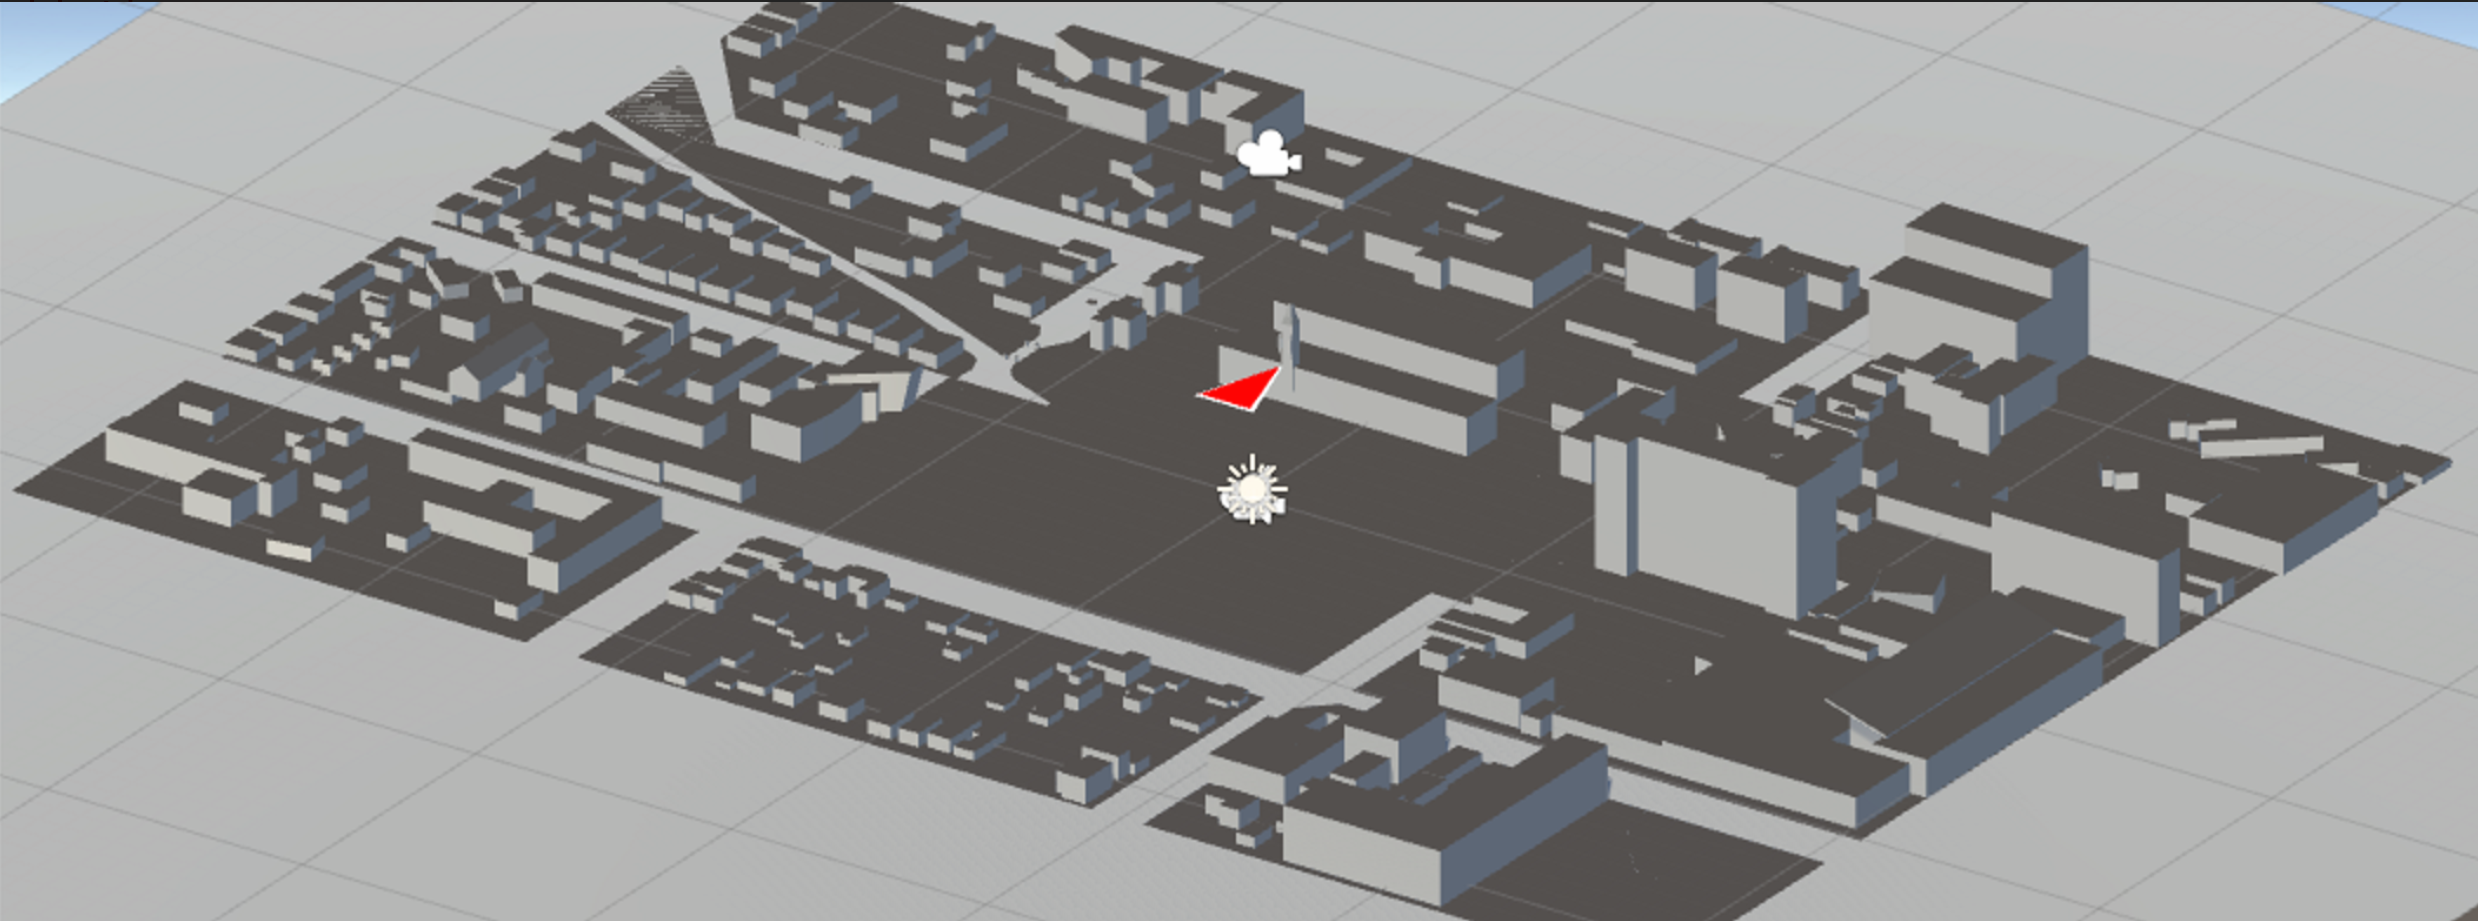
\includegraphics[width=0.7\linewidth]{figures/urban_district}
	\caption{Simulated urban district for the \gls{wa} study}
	\label{fig:urbandistrict}
\end{figure}


\paragraph{Apparatus} The same, as in \ref{study_two}.

% Study Factors and Conditions: what my factors are, conditions == independent variables' values
% + Repeated-measures design?
\paragraph{Study design}
%\textit{Experimental Design} 
The study examined one independent variable: type of awareness presentation. 3 controlled awareness presentations  were made available to the participants: a minimap of the district (\ref{fig:minimap_controller}), auditory cues emitted by translating buildings in the scene (sound of concrete sliding on concrete), and their combination. Awareness presentations were rotated for each participant, so that each presentation was seen in the same position equal number of times. 
Each awareness presentation was tested for 10 minutes, during which exactly 8 buildings were chosen and translated randomly. There were 24 data points measured per user in each session. Data collected were the reaction speed in determining the position of a moving \gls{vb}, along with 3D drawings created by participants.

\begin{figure}[h]
	\centering
	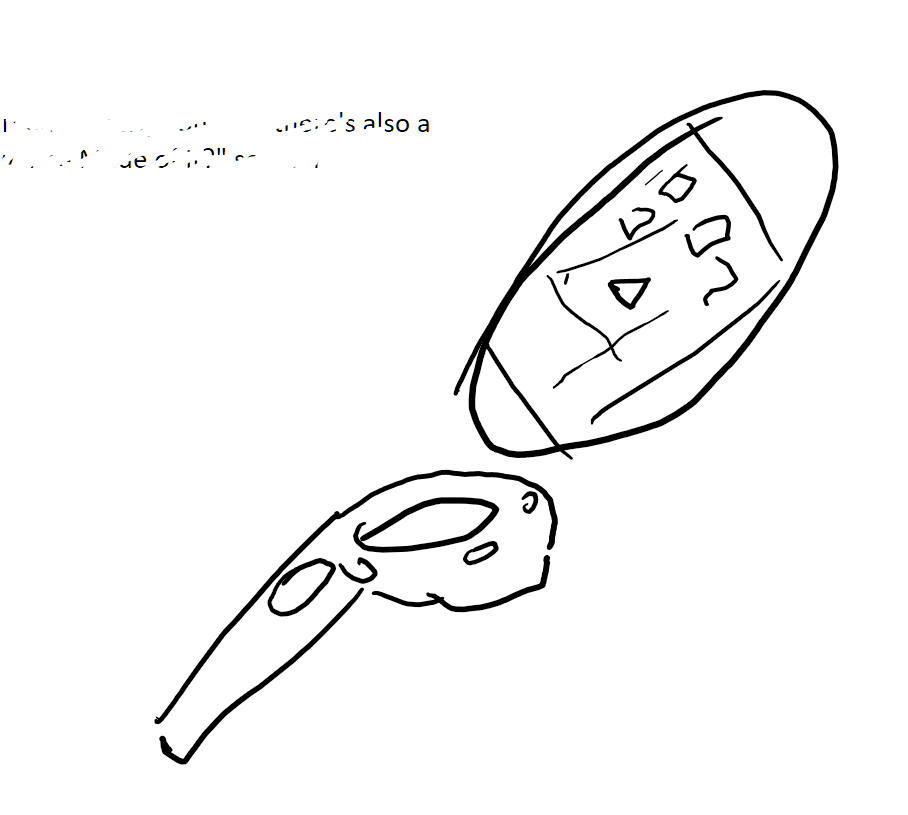
\includegraphics[width=0.7\linewidth]{figures/placeholders/minimap_controller}
	\caption{Controller with the minimap}
	\label{fig:minimap_controller}
\end{figure}


\paragraph{Gutwin vs our study}
% TODO: add a pic: Gutwin's (vertical) and our (horizontal) working (sound) plane
Since, this study extends upon \cite{gutwin_chalk_2011}, in this paragraph I provide a comparison of the two.
The main difference between - workspace is no longer a 2D plane, but an immersive 3D \gls{vr} environment. An important change here is the fact that participants are able to look around at the workspace, and notice some changes to the environment, even without the help of the minimap or auditory cues.
Second distinction is in the primary task of the participant and the simulated agent. In \cite{gutwin_chalk_2011} the participant performs the same task, as an agent: drawing with chalk. Additionally, the participant's actions emit the same sound (even though, at a lower volume) as the drawings of the agent. In this study, the primary task of the participant is - 3D drawing with voxels. This activity doesn't emit any sound. It is also different from the agent's task - translation of buildings in the urban district. Nevertheless, the tasks are still contextually related with regards to the architectural activity in urban environment.
\cite{gutwin_chalk_2011} do not specify the audio plane, in which the sound was simulated, in this experiment, the place was horizontal (TODO: ref figure). 

\begin{figure}[h]
	\centering
	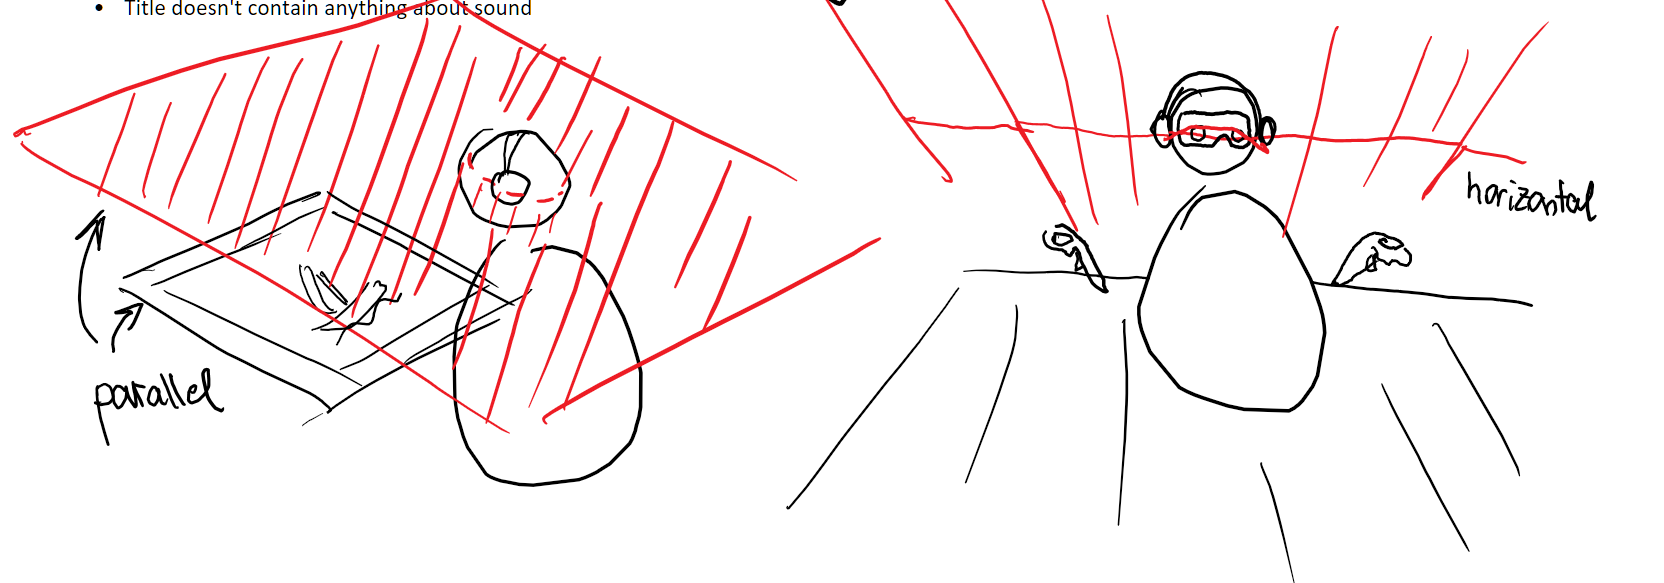
\includegraphics[width=0.7\linewidth]{figures/gutwin_vs_my_study_sound_plane}
	\caption{\cite{gutwin_chalk_2011} sound plane vs this study}
	\label{fig:gutwinvsmystudysoundplane}
\end{figure}


\begin{table}[]
  \caption{Study comparison: \cite{gutwin_chalk_2011} vs \gls{wa} in Immersive \gls{vr}}
  \label{table:study_comp}
  \begin{tabular}{|l|l|l|}
  \hline
                             & \cite{gutwin_chalk_2011}                & This study           \\ \hline
  Workspace dimensions				 & 2D									   & 3D \\ \hline
  Primary (distraction) task & The same as the primary for the simulated actor & Contextually related \\ \hline
  Working (sound) plane      & Variable             & Horizonatal          \\ \hline
  Sound type                 & Auditory icons        & Auditory icons       \\ \hline
  Object of analysis         & Workspace awareness   & Workspace Awareness  \\ \hline
  \end{tabular}
\end{table}

\paragraph{Results}

\paragraph{Discussion}

\subparagraph{Limitations}
% the fact that we only sample the level 1 SA/WA (we won't be going into sampling direction of translation guesses from the participants)
% could also try to describe it according to WA framework
% frame drop
